\documentclass{amsbook}
\usepackage{ytableau,tkz-graph,graphicx,amssymb,hyperref}
\newcommand{\vv}{\mathbf v}
\newcommand{\xx}{\mathbf x}
\newcommand{\yy}{\mathbf y}
\newcommand{\cc}{\mathbf c}
\newcommand{\bb}{\mathbf b}
\renewcommand{\aa}{\mathbf a}
\newcommand{\supp}{\mathrm{supp}}
\newcommand{\RR}{\mathbf R}
\newcommand{\MM}{\mathbf M}
\newcommand{\NN}{\mathbf N}
\newcommand{\ZZ}{\mathbf Z}
\newtheorem{theorem}{Theorem}[section]
\newtheorem{lemma}[theorem]{Lemma}
\newtheorem{corollary}[theorem]{Corollary}
\theoremstyle{definition}
\newtheorem{definition}[theorem]{Definition}
\theoremstyle{remark}
\newtheorem{example}[theorem]{Example}
\newtheorem{exercise}[theorem]{Exercise}
\newtheorem{remark}[theorem]{Remark}
\begin{document}
\title{Linear Programming in Combinatorics}
\author{Amritanshu Prasad}
\address{The Institute of Mathematical Sciences, Chennai.}
\address{Homi Bhabha National Institute, Mumbai.}
\email{amri@imsc.res.in}
\date{\today}
\maketitle
\chapter{Introduction to Linear Programming}
\label{cha:intro-lp}
An excellent reference for the material in this section is the book of G\"artnet and Matousek \cite{GM}.
\section{Feasibility and Optimization}
\label{sec:feas-opt}
A \emph{linear program in equational form} consists of a set of variables $\xx=(x_1,\dotsc,x_n)$, an $m\times n$ matrix $A$ with real entries, a bound vector $\bb=(b_1,\dotsc,b_m)$, and an objective vector $\cc = (c_1,\dotsc,c_n)$.
The \emph{linear program} is the problem:
\begin{equation}
  \tag{LP}
  \label{eq:lp-problem}
  \text{maximize $\cc^T\xx$ subject to $\xx\geq 0$ and $A\xx=\bb$}.
\end{equation}
The set
\begin{displaymath}
  P(A,\bb) = \{\xx\in \RR^n\mid \xx\geq 0,\;A\xx=\bb\}
\end{displaymath}
is called the polytope of all \emph{feasible solutions} to \eqref{eq:lp-problem}.
The function $\xx\mapsto \cc^T\xx$ is called the \emph{objective function}.
An \emph{optimal solution} is a vector $\xx_0\in P(A,\bb)$ such that $\cc^T\xx\leq \cc^T\xx_0$ for every $\xx\in P(A,\bb)$.
Sometimes we will only be interested in the set $P(A,\bb)$ of feasible solutions, which does not depend on the objective vector.

Assume that $\bb$ lies in the column space of $A$ (for otherwise, we would have $P(A,\bb)=\emptyset$), and that the rows of $A$ are linearly independent (if not, we could discard redundant rows to achieve this).
For a subset $B\subset [n]$, let $A_B$ denote the submatrix of $A$ consisting of columns from $B$.
We say that $B$ is a \emph{basic set} if $B$ has $m$ elements and $A_B$ has rank $m$.
For $\xx\in \RR^n$ define:
\begin{displaymath}
  \supp(\xx)=\{1\leq j\leq n\mid x_j\neq 0\}.
\end{displaymath}
\begin{definition}
  [Basic feasible solution]
  A \emph{basic feasible solution} to \eqref{eq:lp-problem} is a feasible solution $\xx\in P(A,\bb)$ such that $\supp(\xx)$ is contained in a basic set.
\end{definition}
Clearly, a feasible solution $\xx$ is basic if and only if the submatrix $A_{\supp(\xx)}$ has linearly independent columns.
\begin{example}[Transportation polytopes]
  \label{example:transportation}
  Take $n=rs$, indexing the $rs$ variables as $\xx=(x_{ij})_{1\leq i\leq r,1\leq j\leq s}$, a rectangular array with $r$ rows and $s$ columns.

  Let $\aa\in \RR_{\geq 0}^r$, and $\bb\in \RR_{geq 0}^s$ be fixed vectors.
  As constraints, say that the row sums and column sums of $\xx$ are specified by the vectors $\aa$ and $\bb$.
  \begin{align}
    \tag{R}
    \label{eq:row-sum-cons}
    \sum_j x_{ij} &= a_i \text{ for } i=1,\dotsc,r,\\
    \tag{C}
    \label{eq:col-sum-cons}
    \sum_i x_{ij} &= b_j \text{ for } j=1,\dotsc,s.
  \end{align}
  These $r+s$ constraints are not independent--the left hand side of the sum of the row sum constraints \eqref{eq:row-sum-cons} is equal to the left hand side of the sum of the column sum constraints~\eqref{eq:col-sum-cons}, being a constraint on the sum of all entries of the matrix.
  If $\sum a_i\neq \sum b_j$, then there are no feasible solutions of this program.
  Thus we assume that the vectors $\aa$ and $\bb$ have equal sums.
  Now, removing, for instance, the last column constraint gives an $(r+s-1)\times rs$ matrix $A$ of rank $r+s-1$, which is equivalent to the original system.
  We will denote the resulting polytope of feasible solutions by $\MM_{\aa\bb}$.
  This polytope is known as the \emph{transportation polytope with margins $(\aa,\bb)$}.
  For an excellent survey on transportation polytopes, see \cite{DLK2014}.

  When $r=s=2$, the constraints can be expressed in matrix form as
  \begin{equation}
    \label{eq:birkhoff2}
    \begin{pmatrix}
      1 & 1 & 0 & 0\\
      0 & 0 & 1 & 1\\
      1 & 0 & 1 & 0
    \end{pmatrix}
    \begin{pmatrix}
      x_{11}\\x_{12}\\x_{21}\\x_{22}
    \end{pmatrix}
    =
    \begin{pmatrix}
      a_1\\a_2\\b_1
    \end{pmatrix}.
  \end{equation}
  Every submatrix of $A$ with three columns is non-singular.
  Thus there are four possible basic sets.
\end{example}
\begin{example}[Birkhoff polytopes]
  \label{example:birkhoff}
  When $r=s$ and $\aa=\bb=(1,\dotsc,1)$, then the resulting polytope is known as the $r$th \emph{Birkhoff polytope}.
  Consider the case where $r=2$, so the constraints are given by \eqref{eq:birkhoff2} with $a_1=a_2=b_1=1$.
  It is easy to see that there are only two basic solutions, given by the permutation matrices:
  \begin{displaymath}
    \begin{pmatrix}
      x_{11} & x_{12}\\
      x_{21} & x_{22}
    \end{pmatrix}
    =
    \begin{pmatrix}
      1 & 0\\
      0 & 1
    \end{pmatrix}, \text{ or }
    \begin{pmatrix}
      x_{11} & x_{12}\\
      x_{21} & x_{22}
    \end{pmatrix}
    =
    \begin{pmatrix}
      0 & 1\\
      1 & 0
    \end{pmatrix}.
  \end{displaymath}
  Each basic feasible solution corresponds to a two possible basic subsets.
\end{example}
\begin{exercise}
  \label{exercise:basic_spanning_trees}
  Let $B$ be a basic subset of $[r]\times [s]$ for the transportation polytope.
  By definition, $B$ has cardinality $r+s-1$.
  Given $B$, define a bipartite graph $\Gamma_B$ on the set $\{1,\dotsc,r\}\sqcup \{1',\dotsc,s'\}$ by joining $i$ to $j'$ if $(i,j)\in B$.
  Show that $\Gamma_B$ is a spanning tree for the complete bipartite graph $K_{r,s}$.
  Show that this construction gives rise to a bijection from the set of basic subsets of $[r]\times[s]$ onto the set of spanning trees of $K_{r,s}$.
\end{exercise}
\begin{exercise}
  Consider the $r$th Birkhoff polytope, $\MM_{(1^r),(1^r)}$.
  Let $\sigma\in S_r$ be a permutation and suppose $\xx$ is the permutation matrix $x_{ij}=\delta_{i\sigma(i)}$.
  Then $\supp(\xx)=\{(i,\sigma_i)\mid i\in [r]\}$.
  The first $r$ rows of the corresponding column vectors of $A$ are just the coordinate vectors of $\RR^r$.
  Therefore each permutation matrix is a basic feasible solution.
  Which spanning trees does it correspond to?
\end{exercise}
\begin{lemma}
  \label{lemma:unique-for-B}
  For each basic subset $B\subset [n]$ of \eqref{eq:lp-problem}, there exists at most one basic feasible solution $\xx$ with $\supp(\xx)\subset B$.
\end{lemma}
In the situation described in the preceding lemma, we say that \emph{$\xx$ is the basic solution corresponding to $B$}.
\begin{proof}
  Let $\xx_B$ denote the vector $(x_i)_{i\in B}$.
  The matrix $A_B$ is non-singular, so the equation $A_B\xx_B=\bb$ has at most one solution.
  Solutions $\xx$ of $A\xx=\bb$ with $\supp(\xx)\subset B$ are in bijection with solutions of $A_B\xx_B=\bb$ (set $x_j=0$ for $j\notin B$ to get $\xx$ from $\xx_B$).
  Therefore $A\xx=\bb$ also has at most one solution.
\end{proof}
\begin{remark}
  The same basic feasible solution could be obtained from different basic sets.
  For example, each basic solution for $r=2$ in Example~\ref{example:birkhoff} corresponds to two basic sets.
  Also not every basic set $B$ admits a basic feasible solution.
  For example, for the $3$rd Birkhoff polytope, $B=\{(1,1),(1,2),(1,3),(2,1),(3,1)\}$ is a basic set with no feasible solution.
\end{remark}
\begin{theorem}
  [Existence of basic optimal solutions]
  \label{theorem:existence-of-basic-solutions}
  For a linear program in equational form:
  \begin{displaymath}
    \text{maximize $\cc^t\xx$ subject to $A\xx=\bb$, $\xx\geq 0$}
  \end{displaymath}
  if there is at least one feasible solution, and the objective function is bounded above on $P(A,\bb)$, then there exists at least one optimal solution.
  Among the optimal solutions there is at least one basic solution.
\end{theorem}
\begin{proof}
  We claim that, for any feasible solution $\xx_0$, there exists a basic feasible solution $\xx$ with $\cc^T\xx\geq \cc^T\xx_0$.
  This implies that an optimal solution, if it exists, will be basic.
  Suppose $\xx$ is a feasible solution.
  Among all feasible solutions $\xx$ with $\cc^T\xx\geq \cc^T\xx_0$ choose one with support of minimal cardinality and call it $\tilde \xx$.
  We will show that $A_{\supp(\tilde\xx)}$ has linearly independent columns, so that $\tilde\xx$ is basic.
  
  Suppose this is not the case.
  Then there exists a vector $\yy\in \RR^n$ with $\supp(\yy)\subset \supp(\xx)$ such that $A\yy=0$.
  Replacing $\yy$ by $-\yy$ if necessary, assume that $\cc^T\yy\geq 0$.

  We claim that we may further assume that $\yy$ has at least one \emph{negative} coordinate.
  Suppose that all the coordinates of $\yy$ are non-negative.
  If $\cc^T\yy=0$, then we can replace $\yy$ with $-\yy$.
  If $\cc^T\yy>0$ and all coordinates of $\yy$ are positive, then $\tilde\xx+t\yy$ is a feasible solution for all $t>0$.
  The objective function $\cc^T(\tilde\xx+t\yy)$ grows unboundedly as $t$ grows, contradicting its boundedness.

  Thus $\yy$ has at least one negative coordinate, hence it is possible to choose a value $t>0$ such that $\tilde\xx+t\yy$ is a feasible solution with $\supp(\tilde\xx+t\yy)\subsetneqq \supp(\tilde\xx)$.
  Since $\cc^T\yy\geq 0$, we have $\cc^T(\tilde\xx+t\yy)\geq \cc^T\tilde\xx$ and $\supp(\tilde\xx+t\yy)$.
  This contradicts the minimality condition on the cardinality of $\supp(\tilde\xx)$.

  The set of basic feasible solutions is finite.
  The element of this set that maximizes the objective function must therefore be an optimal solution.
\end{proof}
\begin{definition}
  [Vertex]
  \label{definition:vertex}
  Let $P\subset \RR^n$ be convex closed set.
  An element $\vv\in P$ is said to be a \emph{vertex} of $P$ if there exists $\cc\in \RR^n$ such that $\cc^T\xx$ attains its maximum \emph{uniquely} at $\vv$.
\end{definition}
Theorem~\ref{theorem:existence-of-basic-solutions} says that every vertex of $P(A,\bb)$ is a basic feasible solution.
The converse is also true:
\begin{theorem}
  The basic feasible solutions to \eqref{eq:lp-problem} are precisely the vertices of $P(A,\bb)$.
\end{theorem}
\begin{proof}
  Let $B\subset [n]$ be a basic subset $\vv$ be the basic feasible solution to \eqref{eq:lp-problem} with respect to $B$.
  Define $\cc$ to be the vector with $c_j=0$ for $j\in B$, and $c_j=-1$ (or any strictly negative number) otherwise.
  Then $\cc^T\vv=0$, and by Lemma~\ref{lemma:unique-for-B}, $\cc^T\xx<0$ for every $\xx\in P(A,\bb)$ different from $\xx_0$.
\end{proof}
\begin{definition}
  [General form of a linear program]
  \label{example:glp}
  A more general form of a linear program involves linear inequalities and equalities.
  As before take $A$ to be an $m\times n$ matrix with real entries, $\bb\in \RR^m$, and $\cc\in \RR^n$.
  A general linear program has the form:
  \begin{equation}
    \label{eq:general-lp}
    \tag{GLP}
    \text{optimize $\cc^T\xx$ subject to }a_{i1}x_1+\dotsb + a_{in}x_n\; R_i\; b_i \text{ for }i=1,\dotsc,m,\; x_jS_j0
  \end{equation}
  where each $R_i$ and $S_j$ is one of the three symbols $\leq$, $\geq$, and $=$, and the word optimize is replaced by either maximize, or minimize.
  A basic feasible solution is one that is defined by equalities in $n$ linearly independent constraints (which could be equality or inequality to begin with).
\end{definition}
\begin{example}
  [Standard equational form of the simplex]
  Consider the linear program in $n$ variables with just one linear equation:
  \begin{displaymath}
    \xx\geq 0;\; x_1+\dotsb+x_n=1.
  \end{displaymath}
  The matrix $A$ in this case has a single row, and rank one.
  The polytope $P(A,1)$ is called the standard $(n-1)$-simplex.
  Every singleton subset of $[n]$ is basic.
  The basic solution corresponding to $B=\{j\}$ is the $i$th coordinate vector $e_j$.
  Given an objective vector $\cc\in \RR^n$, the optimal solution is $e_j$ where $j$ is any of the indices for which $c_j$ is maximal among the coordinates of $\cc$.
\end{example}
\begin{example}
  The cube can be defined by the inequalities:
  \begin{displaymath}
    0\leq x_i \leq 1, \text{ for } i=1,2,3.
  \end{displaymath}
  The inequality $x_i\leq 1$ can be turned into an equality by introducing \emph{slack variables} $y_i$, and writing:
  \begin{displaymath}
    x_i\geq 0,\;y_i\geq 0,\;x_i+y_i\leq 1 \text{ for }i=1,2,3.
  \end{displaymath}
  The linear program in equational form is equivalent to the original, more general one, in the sense that there is a bijection amongst their feasible solutions that maps vertices to vertices (why?).
  What are the basic subsets? What are the basic feasible solutions?
\end{example}
\begin{exercise}
  [The simplex in terms of inequalities]
  The $n$-simplex can also be expressed in terms of inequalities:
  \begin{displaymath}
    \Delta_n = \{(x_1,\dotsc,x_n)\mid 0\leq x_1\leq x_2 \leq \dotsb x_n\leq 1\}.
  \end{displaymath}
  Rewrite this in equational form.
  Determine the basic sets and basic solutions.
\end{exercise}
\begin{exercise}
  Express the hyperoctahedron:
  \begin{displaymath}
    H_n = \{\xx\mid -1\leq x_1+\dotsb+x_n\leq 1\}
  \end{displaymath}
  in equational form.
\end{exercise}

\section{Simplex Tableaus}
\label{sec:simplex-method}

The simplex method begins with a basic set $B$ for which there exists a basic feasible solution.
Let $\bar B=[n]-B$, the complement of $B$ in $[n]$.
Using the relations imposed by $A\xx=\bb$, each of the basic variables $x_j$, $j\in B$, can be expressed in terms of the non-basic variables $x_j$, $j\in \bar B$.
Using this, the objective function can also be expressed in terms of the non-basic variables.

To do this explicitly, note that the system of equations $A\xx=\bb$ can be rearranged as:
\begin{equation}
  \label{eq:basic_from_nonbasic}
  A_B\xx_B = \bb-A_{\bar B}\xx_{\bar B}.
\end{equation}
Here $\xx_B\in\RR^m$ and $\xx_{\bar B}\in\RR^{m-n}$ are vectors whose coordinates are those coordinates of $\xx$ whose indices lie in $B$ and $\bar B$ respectively. 
Since $A_B$ is invertible, the basic variables can be expressed in terms of the non-basic ones:
\begin{displaymath}
  \xx_B = A_B^{-1}(\bb-A_{\bar B}\xx_{\bar B}).
\end{displaymath}
Indeed, the basic feasible solution is computed by setting $\xx_{\bar B}=0$ in the above equation.
If $A_B^{-1}\bb\geq 0$, then it is the basic feasible solution corresponding to $B$.
Othewise there is no basic feasible solution corresponding to $B$.
Since each basic variable is expressed in terms of the non-basic variables in \eqref{eq:basic_from_nonbasic}, the objective function can be expressed in terms of the non-basic variables only:
\begin{displaymath}
  \cc^T\xx = \cc_B^T\xx_B + \cc_{\bar B}^T\xx_{\bar B} = \cc^T_BA_B^{-1}(\bb-A_{\bar B}\xx_{\bar B}) + \cc^T_{\bar B}\xx_{\bar B}.
\end{displaymath}

Thus \eqref{eq:lp-problem} is represented in terms of a \emph{simplex tableau}:
\begin{equation}
  \tag{T}
  \label{eq:tableau}
  \begin{matrix}
    \xx_B & = & \mathbf d - D\xx_{\bar B}\\
    \hline
    \cc^T\xx & = & e - \mathbf e^T \xx_{\bar B},
  \end{matrix}
\end{equation}
the equations above the line being the constraints, and the objective function $\cc^T\xx$ below the line to be maximized.
Here:
\begin{align*}
  \mathbf d & = A_B^{-1}\bb\\
  D & = A_B^{-1}A_{\bar B}\\
  e & = \cc_B^T \mathbf d\\
  \mathbf e^T & = \cc_B^TD - \cc_{\bar B}^T.
\end{align*}
The information contained in \eqref{eq:tableau} is equivalent to the information in \eqref{eq:lp-problem}.
But \eqref{eq:tableau} gives a parametrization of $P(A,b)$ in terms of a subset of $\RR^{n-m}$.
\begin{theorem}
  \label{theorem:basic-parametrization}
  For every basic subset $B\subset [n]$ in the linear program \eqref{eq:lp-problem},
  \begin{equation}
    \tag{$*$}
    \label{equation:tableau-par}
    P(A,\bb) = \{\xx\in \RR^n\mid \xx_B=A_B^{-1}(\bb-A_{\bar B}\xx_{\bar B})\geq 0,\;\xx_{\bar B}\geq 0\}.
  \end{equation}
  In other words, \eqref{eq:tableau} gives a parametrization of $P(A,\bb)$ in terms of the polytope:
  \begin{displaymath}
    P_B(A,\bb) = \{\xx_{\bar B}\in \RR_{\geq 0}^{n-m}\mid A_B^{-1}(\bb-A_{\bar B}\xx_{\bar B})\geq 0\}\subset \RR^{n-m}.
  \end{displaymath}
\end{theorem}
\begin{proof}
  The conditions $A\xx=\bb$ and $\xx_B=A_B^{-1}(\bb-A_{\bar\xx}x_{\bar B})$ are equivalent.
\end{proof}
\begin{example}
  \label{example:birkhoff3-tableau}
  Consider the Birkhoff polytope (Example~\ref{example:birkhoff}) for $r=3$.
  For convenience we abbreviate the variable indices $(i,j)$ to $ij$.
  The matrix $A$ has columns indexed by pairs in $[d]\times [d]$ written in increasing lexicographic order:
  \begin{displaymath}
    A =
    \begin{pmatrix}
      1 & 1 & 1 & 0 & 0 & 0 & 0 & 0 & 0\\
      0 & 0 & 0 & 1 & 1 & 1 & 0 & 0 & 0\\
      0 & 0 & 0 & 0 & 0 & 0 & 1 & 1 & 1\\
      1 & 0 & 0 & 1 & 0 & 0 & 1 & 0 & 0\\
      0 & 1 & 0 & 0 & 1 & 0 & 0 & 1 & 0\\
    \end{pmatrix}
  \end{displaymath}
  Fix as objective function $x_{11}+x_{22}+x_{33}$.
  A basic subset is $B=\{11,12,13,22,31\}$ with basic solution given by $x_{13}=x_{22}=x_{31}=1$, and all other coordinates zero.
  The corresponding simplex tableau is:
  \begin{displaymath}
    \begin{matrix}
      x_{11} & = & -x_{21} +x_{32}+x_{33}\\
      x_{12} & = & x_{21}+x_{23}-x_{32}\\
      x_{13} & = & 1-x_{23}-x_{33}\\
      x_{22} & = & 1-x_{21} -x_{23}\\
      x_{31} & = & 1-x_{32}-x_{33}\\
      \hline
      \cc^T\xx & = & 1-2x_{21}-x_{23}+x_{32}+2x_{33}.
    \end{matrix}
  \end{displaymath}
  In the above example, the objective function can be increased by increasing $x_{32}$ or $x_{33}$, the variables with positive coefficients in the last row of the tableau.
  However, this increase should respect the constraints that all the variables are non-negative.
  The condition $x_{12}\geq 0$ (using the second equation, and leaving the values of $x_{21}$ and $x_{23}$ unchanged at $0$) gives $x_{32}\leq 0$.
  Therefore, it is not feasible to increase $x_{32}$.
  However, it is feasible to increase $x_{33}$.
  The conditions $x_{13}\geq 0$ and $x_{31}\geq 0$ give $x_{33}\leq 1$.
  So we set $x_{33}=1$, and recalculate all the basic variables, getting $x_{11}=x_{22}=x_{33}=1$, and all other variables $0$.
  We move $x_{33}$ to the set of basic variables, and move $x_{13}$ to the set of non-basic (which has now become $0$), and use the equation:
  \begin{displaymath}
    x_{33}=1-x_{13}-x_{23}.
  \end{displaymath}
  Using this we get a new tableau:
  \begin{displaymath}
    \begin{matrix}
      x_{11} & = & 1-x_{21} +x_{32}+x_{23}-x_{13}\\
      x_{12} & = & x_{21}+x_{23}-x_{32}\\
      x_{22} & = & 1-x_{21} -x_{23}\\
      x_{31} & = & x_{13}+x_{23}-x_{32}-x_{33}\\
      x_{33} & = & 1-x_{23}-x_{13}\\
      \hline
      \cc^T\xx & = & 3-2x_{13}-2x_{21}-3x_{23}+x_{32}.
    \end{matrix}
  \end{displaymath}
  All the non-basic variables have negative coefficients, except $x_{32}$.
  However, the constraint $x_{12}\geq 0$ still does not allow us to increase $x_{32}$ without changing any other non-basic variable.
  This suggests that we may have arrived at a maximum value for the objective function.
  Indeed, $x_{12}=x_{21}+x_{23}-x_{32}\geq 0$ implies that $x_{32}\leq x_{21}+x_{23}$ for every $\xx\in P(A,\bb)$, whence
  \begin{displaymath}
    \cc^T\xx=3-2x_{13}-2x_{21}-3x_{23}+x_{32}\leq 3-2x_{13}-x_{21}-2x_{23}\leq 3.
  \end{displaymath}
  Therefore $3$ is indeed a global maximum for the objective function, and is obtained uniquely at $x_{ij}=\delta_{ij}$.

  An alternative approach would be to induct $x_{32}$ into the set of basic variables, and remove $x_{12}$.
  Now the basic set is changed to $\{11,22,31,32,33\}$, but the basic feasible solution remains unchanged.
  This will result in the tableau:
  \begin{displaymath}
    \begin{matrix}
      x_{11} & = & 1-x_{12}+x_{32}+2x_{23}-x_{13}\\
      x_{22} & = & 1-x_{21} -x_{23}\\
      x_{31} & = & x_{12}+x_{13}-x_{21}-x_{33}\\
      x_{32} & = & x_{21}+x_{23}-x_{12}\\
      x_{33} & = & 1-x_{23}-x_{13}\\
      \hline
      \cc^T\xx & = & 3-2x_{13}-x_{21}-2x_{23}-x_{12}.
    \end{matrix}
  \end{displaymath}
  In this case, all the coefficients of the objective function, when expressed in terms of non-basic variables, are negative.
  Theorem~\ref{theorem:basic-parametrization} then implies that $x_{ij}=\delta_{ij}$ is the unique global maximum.
\end{example}
More generally Theorem~\ref{theorem:basic-parametrization} gives:
\begin{theorem}
  \label{theorem:pivot-basic}
  Let $B$ be a basic set for \eqref{eq:lp-problem}.
  Suppose that the objective function, when expressed in terms of the non-basic variables as in the last line of the tableau \eqref{eq:tableau} has all coefficients nonpositive.
  Then the basic feasible solution $\xx_0$ corresponding to $B$ is a solution to \eqref{eq:lp-problem}.
  If all the non-basic variables occur with strictly negative coefficients, then $\xx_0$ is the unique solution to \eqref{eq:lp-problem}.
\end{theorem}

\section{Pivot Rules}
\label{sec:pivot-rules}

Given a basic subset $B$ for the linear program \eqref{eq:lp-problem}, consider the corresponding tableau \eqref{eq:tableau}.
Assume also that $B$ admits a basic feasible solution $\xx$.
Suppose that $e_k>0$ for some $k\in \bar B$.
For each $i$ in $B$, we have:
\begin{equation}
  \label{eq:bound-i}
  x_i = d_i - \sum_{j\in \bar B} D_{ij}x_j.
\end{equation}
The constraint $x_i\geq 0$ can be rewritten as:
\begin{displaymath}
  D_{ik}x_k \leq d_i - \sum_{j\in \bar B,\;j\neq k} D_{ij}x_j.
\end{displaymath}
Since $B$ admits a basic feasible solution where all the basic variables are zero, we have $d_i\geq 0$.
If $D_{ik}\leq 0$, then $x_k$ can be increased without bound without violating \eqref{eq:bound-i}.
If, on the other hand, $D_{ik}>0$, then $x_k$ can be increased up to $d_i/D_{ik}$.
Therefore, we can increase $x_k$ up to $m=\min\{d_i/D_{ik}\mid i\in B, D_{ik}>0\}$.
In general $m\geq 0$, and it is quite possible (as we have seen in Example~\ref{example:birkhoff3-tableau}) that $m=0$.
Let $l$ be any index for which $m=d_l/D_{il}$.
Let $B'=B\cup\{k\}-\{l\}$.

We have an expression for $x_k$ in terms of the variables $\{x_j\mid j\in \bar B'\}$:
\begin{equation}
  \label{eq:pivot-sub}
  x_k = D_{lk}^{-1}(d_l-x_l-\sum_{j\in \bar B\;j\neq k} D_{lj}x_j).
\end{equation}
This can be substituted into the equations \eqref{eq:bound-i} for all $i\in B-\{l\}$ to write $x_i$ in terms of the variables $\{x_j\mid j\in \bar B'\}$.
Thus each variable $x_i$, for $i\in B'$ can be expressed in terms of the variables $\{x_j\mid j\in \bar B'\}$.
Also, the substitution \eqref{eq:pivot-sub} can be used to express the objective function in terms of the variables $\{x_j\mid j\in \bar B'\}$.
Let $\xx'$ be the vector obtained from $\xx$ by changing $x_k$ to $m$, and $x_l$ to $0$.
\begin{lemma}
  If $B$ is a basic subset with basic feasible vector $\xx$ and $B'$ and $\xx'$ are obtained from $B$ and $\xx$ as described above, then $B'$ is also a basic subset, and $\xx'$ is a basic feasible solution corresponding to $B'$.
\end{lemma}
\begin{proof}
  Since $B$ is a basic subset, the analysis at the beginning of Section~\ref{sec:simplex-method} shows that the equations:
  \begin{displaymath}
    A\xx=\bb \text{ and } \xx_B = \mathbf d - D\bar \xx_{\bar B} 
  \end{displaymath}
  are equivalent.
  Our choices of $k$ and $l$ above ensure that these equations are further equivalent to
  \begin{displaymath}
    \xx_{B'} = \mathbf d' - D'\bar \xx_{\bar B'},
  \end{displaymath}
  for some vector $\mathbf d'$ and some matrix $D'$.
  Setting $\xx_{\bar B'}=0$ says that there is a unique value for $\xx_{B'}$ such that, if $\xx''\in \RR^n$ is obtained from $\xx_{B'}$ by setting the coordinates in $\bar B'$ to $0$, then $A\xx''=\bb$.
  In other words, $A_{B'}\xx_{B'}=\bb$ has a unique solution.
  It follows that $A_{B'}$ is non-singular, and so $B'$ basic.
  By Lemma~\ref{lemma:unique-for-B}, the vector $\xx''$ constructed in this proof coincides with the vector $\xx'$ constructed earlier, so the rest of the lemma also follows.
\end{proof}
\begin{definition}
  [Pivot step]
  \label{definition:pivot}
  Given a basic subset $B\subset[n]$ and the corresponding tableau \eqref{eq:tableau} for a linear program \eqref{eq:lp-problem}, a \emph{leaving variable} is any variable $x_k$ such that $k\in \bar B$, and $e_k>0$.
  Let $m=\min\{d_i/D_{ik}\mid D_{ik}>0\}$.
  Assume that $m<\infty$ (we will come to the case $m=\infty$ shortly).
  Having picked a leaving variable $x_k$, an \emph{entering variable} is any variable $x_l$ such that $m=d_l/D_{lk}$.
  A pivot step is a change of basic set $B\mapsto B':=B\cup\{x_l\}-\{x_k\}$, where $x_l$ is an entering variable and $x_k$ is a leaving variable.
  By Theorem~\ref{theorem:pivot-basic}, $B'$ is again a basic subset for \eqref{eq:lp-problem}.
  If $\xx$ is the basic feasible solution corresponding $B$, and $\xx'$ is the basic feasible solution corresponding to $B'$, then $\cc^T\xx'\geq \cc^T\xx$.
\end{definition}
In what situation is there no possible pivot step?
The first possibility is that $e_k\leq 0$ for all $k\in \bar B$.
Then Theorem~\ref{theorem:pivot-basic} tells us that the basic feasible solution corresponding to $B$ is maximizes the objective function of $P(A,\bb)$.
Another possibility is that, for some $k\in\bar B$ such that $e_k>0$, $D_{ik}<0$ for all $i\in B$.
Then, starting with the basic feasible solution corresponding to $B$, $x_k$ can be increased unboundedly without disturbing any of the other non-basic variables (which are set to $0$) without making any of the variable $x_i$, $i\in B$ negative.
This shows that the objective function $\cc^T\xx$ is unbounded on $P(A,\bb)$.
If neither of these cases occur, then a pivot step $B\mapsto B'$ is possible.
However, it is quite possible that $m=0$ (this happened with the variable $x_{32}$ in Example~\ref{example:birkhoff3-tableau}).
In this case the pivot step $B\mapsto B'$ happens, but $\xx'=\xx$.
Of course, the value of the objective function remains unchanged.
Also, $\supp(\xx)=\sup(\xx')\subset B\cap B'\subsetneq B$.
\begin{definition}
  [Degenerate basic subset]
  A basic subset for \eqref{eq:lp-problem} is said to be \emph{degenerate} if it admits a basic feasible solution $\xx$ such that $\supp(\xx)\subsetneq B$.
\end{definition}
\begin{lemma}
  Given an $m\times n$ matrix $A$, the set of constraint vectors $\bb\in \RR^n$ for which there exist degenerate basic subsets is a finite union of hyperplanes.
\end{lemma}
\begin{proof}
  If $B\subset [n]$ is degenerate, then the vector $A_B^{-1}\bb$ lies in the union of coordinate hyperplanes.
  In other words, $\bb$ lies in image under $A_B$ of a coordinate hyperplane, which, by the non-singularity of $A_B$, is a hyperplane.
  Thus the set of constraint vectors $\bb$ for which there exists a degenerate basic subset is a finite union of a hyperplanes.
\end{proof}
\begin{example}
  [Degeneracy in transportation polytopes]
  When are the defining equations for $\MM_{\aa\bb}$ from Example~\ref{example:transportation} degenerate?
  Suppose that $\xx$ is a basic feasible solution corresponding to a basic subset $B$.
  If $\supp(\xx)\subsetneq B$, then $\Gamma_{\supp\xx}$ is a forest with at least two connected components.
  Therefore there exist proper subsets $K\subset [r]$ and $L\subset [s]$ with complements $[r]-K$ and $[s]-L$ respectively such that $\Gamma_{\supp\xx}$ has no edges between $K$ and $\bar L$ or between $\bar K$ and $L$.
  It follows that
  \begin{displaymath}
    \sum_{i\in K} a_i = \sum_{i\in K}\sum_{j\in L} x_{ij} = \sum_{j\in L} b_j.
  \end{displaymath}
  Conversely suppose there exist proper subset $K\subset [r]$ and $L\subset [s]$ such that
  \begin{equation}
    \label{eq:transportation-degeneration}
    \sum_{i\in K}a_i = \sum_{j\in L} b_j,
  \end{equation}
  then (as we shall see in Theorem~\ref{theorem:brualdi-algo}) both $\MM_{\aa_K\bb_L}$ and $\MM_{\aa_{\bar K}\bb_{\bar L}}$ are non-empty.
  Putting together feasible points for these polytopes will with give us a point $\xx$ in $\MM_{\aa\bb}$ whose support is a forest, hence a proper subset of any basic subset.
  Thus we have the following:
  \begin{theorem}
    Assume that $\aa>0$ and $\bb>0$.
    The polytope $\MM_{\aa\bb}$ is degenerate if and only if there exist proper subsets $K\subset [r]$ and $L\subset [s]$ such that the condition \eqref{eq:transportation-degeneration} holds.
  \end{theorem}
\end{example}
Since a finite union of coordinate hyperplanes is a nowhere dense subset of $\RR^n$, it is very unlikely that degeneracy will occur in a real-world linear programming problem.
Moreover, if it does occur, a small enough perturbation of $\bb$ will bring us back to the non-degenerate world while giving the correct basic subset whose basic feasible solution also optimizes the original problem.
\begin{definition}[Non-degenerate linear program]
  We say that \eqref{eq:lp-problem} is non-degenerate if it admits no degenerate basic subset $B\subset[n]$.
\end{definition}
\begin{theorem}
  Assume that \eqref{eq:lp-problem} is a non-degenerate linear program.
  Starting with any basic set $B$, a finite number of pivot steps (Definition~\ref{definition:pivot}) will result in a basic set whose basic feasible solution is optimal, or else establish that the objective function is unbounded on $P(A,\bb)$.
\end{theorem}
\begin{proof}
  Indeed, non-degeneracy ensures that the objective function increases strictly at each pivot step or $m=\infty$.
  If $m=\infty$ at any pivot step, then the objective function is unbounded.
  Otherwise, becuase the objective function increases strictly, no basic subset is ever repeated in a run of the algorithm.
  Since there are only finitely many possible basic subsets, the algorithm must halt at an optimal solution.
\end{proof}
The number of basic subsets can grow exponentially with the number of variable.
In an implementation of a linear programming algorithm a rule for choosing the leaving variable and the entering variable has to be specified.
Such a rule is called a \emph{pivot rule}.
For a discussion of commonly used pivot rules, their relative merits and demerits, the reader is referred to \cite[Section~5.7]{GM}.

However, degeneracy is ubiquitous in combinatorial applications of linear programming.
For example, \emph{every} basic subset for the $r$th Birkhoff polytope for every $r>1$ either does not admit a basic feasible solution, or is degenerate, since every vertex of the Birkhoff polytope is a permutation matrix.
Moreover, the support of any permutation matrix has $r$ elements, but every basic subset has cardinality $2r-1$.
\begin{example}
  Consider the Birkhoff polytope for $r=3$ with objective function:
  \begin{displaymath}
    x_{12}+x_{13}+x_{21}+x_{23}+x_{31}+x_{32}.
  \end{displaymath}
  For $B=\{11,12,13,22,33\}$, the tableau is
  \begin{displaymath}
    \begin{matrix}
      x_{11}&=&1-x_{21}-x_{31}\\
      x_{12}&=&x_{21}+x_{23}-x_{32}\\
      x_{13}&=&-x_{23}+x_{31}+x_{32}\\
      x_{22}&=&1-x_{21}-x_{23}\\
      x_{33}&=&1-x_{31}-x_{32}\\
      \hline
      \cc^T\xx&=&2x_{21}+x_{23}+2x_{31}+x_{32}.
    \end{matrix}
  \end{displaymath}
  All four non-basic variables have positive coefficients in the objective function.
  Using $x_{23}$ or $x_{32}$ as entering variables leads to pivots that do not increase the objective function.
\end{example}
The simplex method begins with a basic subset $B\subset [n]$ for \eqref{eq:lp-problem}.
How does one find a basic subset to begin with?
Indeed, the total number of subsets of $[n]$ is $2^n$, and finding a basic subset could be like finding a needle in a (albeit finite) haystack.
The trick is to start with an infeasible point (usually $\xx=0$), quantify its ``infeasibility'' and then move to a feasible point (if it exists) by taking the negative of this infeasibility as an objective function.

So, introduce variables $x_{n+1},\dotsc,x_{n+m}$, all constrained to take non-negative values.
The variable $x_{n+i}$ will measure the feasibility gap in the $i$th equation:
\begin{displaymath}
  a_{i1}x_1+\dotsb+a_{in}x_n+\mathrm{sgn}(b_i)x_{n+i}=b_i,
\end{displaymath}
and then maximize $-x_{n+1}-x_{n+1}-\dotsb-x_{n+m}$.
In other words, the auxilliary linear program has coefficient matrix $\tilde A = \begin{pmatrix}A & I_m\end{pmatrix}$ in block form, where $I_m$ denotes the $m\times m$ identity matrix.
The bound vector $\bb$ remains unchanged.
The objective vector is $(0,\dotsc,0,-1,\dotsc,-1)$ (with $n$ zeros and $m$ $-1$'s).
In this case $B=\{n+1,\dotsc,n+m\}$ is clearly a basic subset with basic feasible solution $\tilde\xx=(0,\dotsc,0,|b_1|,\dotsc,|b_m|)$.
The original program \eqref{eq:lp-problem} has a feasible solution if and only if the maximum value of the objective function is $0$.
Thus locating a basic subset is itself a linear programming problem with an obvious basic subset.
\begin{example}
  [Construction of transportation arrays]
  \label{example:transportation-vertex-algo}
  In order to construct an $m\times n$ transportation array with margins $\aa$ and $\bb$ (Example~\ref{example:transportation}), we introduce $r+s$ auxilliary variables $u_1,\dotsc,u_r$ and $v_1,\dotsc,v_s$.
  Consider the auxilliary linear program:
  \begin{equation}
    \label{eq:transportation}
    \begin{matrix}
      \sum_{j=1}^s x_{ij} + u_i & = a_i \text{ for } 1\leq i\leq r,\\
      \sum_{i=1}^r x_{ij} + v_j & = b_j \text{ for } 1\leq j\leq s,\\
      x_{ij}\geq 0,\;u_i\geq 0\;v_j\geq 0 &= \text{ for } 1\leq i\leq r,\;1\leq j\leq s,\\
      \hline
      \text{maximize} & -u_1-\dotsb -u_r - v_1 - \dotsb -v_s.
    \end{matrix}
  \end{equation}
  This auxilliary program comes with a God-given basic variables $\{u_1,\dotsc,u_r,v_1,\dotsc,v_s\}$.
  The corresponding tableau is:
  \begin{displaymath}
    \begin{matrix}
      u_i & = a_i - \sum_{j=1}^s x_{ij} \text{ for } i=1,\dotsc,r,\\
      v_j & = b_j - \sum_{i=1}^r x_{is} \text{ for } j=1,\dotsc,s,\\
      \hline
      \cc^T\xx &= -\sum a_i - \sum_j b_j + \sum_i\sum_j x_{ij}. 
    \end{matrix}
  \end{displaymath}
  We may choose any $x_{ij}$ as entering variable.
  Then the leaving variable will be $u_i$ if $a_i<b_j$, and $v_j$ if $b_i<u_j$.
  If $a_i=b_j$ either variable could be chosen as leaving.
  We now have a new tableau, for example if we had chosen $x_{i_0j_0}$ as entering $u_{i_0}i$ as leaving,
  \begin{displaymath}
    \begin{matrix}
      x_{i_0j_0} & = a_{i_0} - u_{i_0} -\sum_{j\neq j_0} x_{i_0j}\\
      v_{j_0} & = b_{j_0} - \sum_{i\neq i_0} x_{ij_0} - a_{i_0} + u_{i_0} + \sum_{j\neq j_0} x_{i_0,j}\\
      u_i & = a_i - \sum_j x_{ij} \text{ for }i\neq i_0,\\
      v_j & = b_j - \sum_{i=1}^r x_{is} \text{ for } j\neq j_0,\\
      \hline
      \cc^T\xx & = -\sum_{i\neq i_0} a_i - \sum b_j + \sum_{i\neq i_0}\sum_jx_{ij} -u_{i_0}. 
    \end{matrix}
  \end{displaymath}
  The variables $x_{i_0,j}$ (the $i_0$th row) have dissapeared from the objective function.
  The $i_0$th row is now saturated and the rest of the algorithm would run with the same set of possible pivot steps as if the $i$th row simply did not exist, and $b_{j_0}=b_j-a_{i_0}$.
  The new margin vectors are:
  \begin{displaymath}
    \aa' = (a_1,\dotsc,a_{i_0-1},a_{i_0+1},\dotsc,a_r),\quad \bb'=(b_1,\dotsc,b_{j_0}-1,b_{j_0}-a_{i_0},b_{j_0+1},\dotsc,b_s).
  \end{displaymath}
  We now analyze the running of this auxilliary program by induction on $r+s$.
  \begin{theorem}
    \label{theorem:brualdi-algo}
    The transportation polytope $\MM_{\aa\bb}$ is non-empty if and only if $\sum_{i=1}^r a_i=\sum_{j=1}^s b_j$.
    If this condition holds, then every basic feasible solution in $\MM_{\aa\bb}$ can be obtained by a sequence of pivot steps for the auxilliary linear program described above.
  \end{theorem}
  The method for finding all the vertices of $\MM_{\aa\bb}$ in the above theorem is equivalent to the algorithm of Corollary~8.1.4 in Brualdi's book \cite{Brualdi}. 
  \begin{proof}
    Clearly if $\MM_{\aa\bb}$ has a feasible point $\xx=(x_{ij})$ then $\sum a_i=\sum_i\sum_j=\sum_jb_j$.
    For the converse, proceed by induction on $r+s$.
    Take as base case $r+s=2$, where the array has one row and one column, and clearly it is feasible if the row margin equals the column margin.
    As we have seen, each pivot step reduces $r+s$ by one, and reduces both the margins by the same quantity.
    Thus by the induction hypothesis the new transportation polytope is non-empty.

    It remains to show that every basic feasible solution can be attained by a sequence of pivot steps.
    Suppose that $\xx$ is a basic feasible solution.
    By Example~\ref{exercise:basic_spanning_trees}, $\Gamma_{\supp\xx}$ is contained in a spanning tree, and hence is a spanning forest.
    Consider a leaf of this graph, say a row index $1\leq i_0\leq r$ (the case where it is a column index is not different).
    Being a leaf, this vertex is connected to a unique column index $1\leq j_0\leq s$.
    Perform the first pivot step for the auxilliary program taking $x_{i_0j_0}$ as entering variable and $u_{i_0}$ as leaving variable.
    As discussed before what remains is a problem with $r-1$ rows and $s$ columns, for which all basic feasible solutions can indeed be obtained by induction hypothesis.
  \end{proof}
\end{example}  
\begin{theorem}
  [Birkhoff von Neumann theorem]
  The vertices of the Birkhoff polytope are permutation matrices.
\end{theorem}
\begin{proof}
  Every permutation matrix, being supported on a forest (in fact a perfect matching) of $K_{n,n}$ is a vertex.
  The converse follows from observing (by induction) that every run of the algorithm of Example~\ref{example:transportation-vertex-algo} produces a permutation matrix.
\end{proof}
\section{Dealing with degeneracy}
\label{sec:deal-with-degen}
In the non-degenrate case, we saw that, with an sequence of arbitrarily chosen pivot moves, it is possible to go from any basic feasible solution to an  optimal one.
In the degenerate case, it is quite possible that we end up repeating a cycle of pivot moves indefinitely.
This can be avoided using \emph{Bland's rule} for choosing the leaving and entering variable.
\begin{definition}
  [Bland's rule]
  Given a basic subset $B\subset [n]$ for \eqref{eq:lp-problem}, choose the incoming variable with minimum possible index, and among all the outgoing variables detrmined by this incoming variable, choose the one with minimum possible index.
\end{definition}
\begin{theorem}
  With Bland's rule, starting with a given basic subset $B\subset [n]$ for \eqref{eq:lp-problem}, it is not possible to return to $B$ after a any number of pivot steps.
\end{theorem}
\begin{proof}
  Suppose that, upon using pivot steps according to Bland's rule, the simplex method encounters a cycle.
  Let $F$ denote the set of all the entering (or leaving variables) in the pivot steps of this cycle.
  Since the objective function does not increase in a cycle, it must be the case that the basic feasible solutions do not change.
  Therefore for all basic feasible solutions in the cycle $x_j=0$ for all $j\in F$.
  
  Let $v$ be the largest index in $F$.
  Let $B$ be a basic subset in the cycle just before $x_v$ enters the basic set.
  Suppose that the simplex tableau corresponding to $B$ is:
  \begin{displaymath}
    \begin{matrix}
      \xx_B & = & \mathbf d - D\xx_{\bar B}\\
      \hline
      \cc^T\xx & = & e - \mathbf e^T \xx_{\bar B},
    \end{matrix}
  \end{displaymath}
  Since we are following Bland's rule, $v$ is the least index among all possible entering variables.
  Therefore for any $j\in F-\{v\}$, since $j<v$, $e_j\leq 0$.

  Let $B'$ be a basic subset in the cycle just before $x_v$ leaves the basic set.
  Suppose that the simplex tableau corresponding to $B'$ is:
  \begin{displaymath}
    \begin{matrix}
      \xx_{B'} & = & \mathbf d' - D'\xx_{\bar B'}\\
      \hline
      \cc^T\xx & = & e' - \mathbf {e'}^T \xx_{\bar B'},
    \end{matrix}
  \end{displaymath}
  Suppose $x_l$ enters the basic set as $v$ leaves it.
  Now for all $j\in F$ $d_j$, being the value of $x_j$ in the basic feasible solution corresponding to $B'$, must be $0$.
  Since we are following Bland's rule, $v$ is the least index among all possible leaving variables.
  Therefore, for any $j\in F-\{v\}$, since $j<v$ and $d'_v/D'_{vk'}=d'_j/D'_{jk'}=0$, we must have $D'_{jk'}<0$.

  To summarize, we have established:
  \begin{gather}
    \label{eq:cycle1}
    \text{$e_v>0$ and for all $j\in F-\{v\}$, $e_j\leq 0$},\\
    \label{eq:cycle2}
    \text{$D_{vk'}>0$ and for all $j\in F-\{v\}$, $D'_{jk'}<0$}.
  \end{gather}

  Now consider the auxilliary linear program:
  \begin{displaymath}
    \text{maximize $\cc^T\xx$ subject to $A\xx=\bb$, $x_v\leq 0$, $\xx_{F-\{v\}}\geq 0$, $\xx_{\bar B-F}=0$.}
  \end{displaymath}
  There is no constraint on the variables $\xx_{B-F}$. They may assume positive or negative signs, or take the value $0$.

  Let $\tilde\xx$ denote the basic feasible solution to \eqref{eq:lp-problem} corresponding to $B$.
  It is also feasible for the auxilliary program.
  The condition \eqref{eq:cycle1} and the constraints on the auxilliary program imply that, for all feasible $\xx$ in the auxilliary program, $e_j\xx_j\leq 0$ for all $j\in \bar B$.
  Therefore, $\tilde\xx$ is optimal.

  Now $\tilde\xx$ is also the basic feasible solution to the auxilliary program corresponding to the basic subset $B'$.
  Since there are no sign constraints on $\xx_{B-F}$, the conditions \eqref{eq:cycle2} imply that, starting with $\tilde\xx$ the leaving variable $x_{k'}$ can be increased indefinitely without violating feasibility.
  Therefore the objective function is unbounded in the auxilliary program.
  This contradicts the earlier assertion that the auxilliary program had an optimal solution.
\end{proof}
\section{Duality}
\label{sec:duality}
Consider a linear program in the form:
\begin{equation}
  \label{eq:lpineq}
  \tag{P}
  \text{maximize $\cc^T\xx$ subject to $A\xx\leq \bb$, $\xx\geq 0$},
\end{equation}
with $n$ variables $\xx=(x_1,\dotsc,x_n)$, $A\in M_{m\times n}(\RR)$, $\bb\in \RR^m$.
We will call \eqref{eq:lpineq} the \emph{primal} program.

The program \emph{dual} to \eqref{eq:lpineq} is defined as:
\begin{equation}
  \label{eq:lpdual}
  \tag{D}
  \text{minimize $\bb^T\yy$ subject to $A^T\yy\geq \cc$, $\yy\geq 0$},
\end{equation}
with $n$ variables $\yy=(y_1,\dotsc,y_n)$.

Suppose $\xx$ and $\yy$ are feasible solutions to \eqref{eq:lpineq} and \eqref{eq:lpdual} respectively.
Then, combining the constraints $\cc^T\leq \yy^TA$ and $A\xx\leq \bb$, along with $\xx\geq$ and $\yy\geq 0$ gives:
\begin{displaymath}
  \cc^T\xx\leq\yy^TA\xx\leq \yy^T\bb.
\end{displaymath}
Thus if \eqref{eq:lpineq} and \eqref{eq:lpdual} are feasible, then the maximum of \eqref{eq:lpineq} is bounded above by the minimum of \eqref{eq:lpdual}.
It follows that if the objective function of \eqref{eq:lpineq} is unbounded above on its feasible set, then \eqref{eq:lpdual} has no feasible solutions.
Similarly, if the objective function of \eqref{eq:lpdual} is unbounded below on its feasible set, then \eqref{eq:lpineq} has no feasible solutions.
\begin{theorem}
  \label{theorem:duality}
  If \eqref{eq:lpineq} and \eqref{eq:lpdual} are both feasible, then the maximum value of \eqref{eq:lpineq} equals the minimum value of \eqref{eq:lpdual}.
\end{theorem}
\begin{proof}
  Convert \eqref{eq:lpineq} to equational form by introducing slack variables $x_{m+1},\dotsc,x_{m+n}$.
  Let $\bar\xx = (x_1,\dotsc,x_{m+n})$, $\bar A=
  \begin{pmatrix}
    A & I_m
  \end{pmatrix}
  $,
  and $\bar\cc=(c_1,\dotsc,c_n,0,\dotsc,0)\in \RR^{m+n}$.
  The equational form of \eqref{eq:lpineq} is
  \begin{displaymath}
    \text{maximize $\bar\cc^T\bar\xx$ subject to $\bar A\bar\xx=\bb$, $\bar\xx\geq 0$}.
  \end{displaymath}
  Let $B\subset [m+n]$ be a basic subset whose basic feasible solution $\bar\xx^*$ maximizes the objective function.
  The corresponding simplex tableau is:
  \begin{equation}
    \label{eq:duality-tab}
    \begin{array}{cc}
      \bar\xx_B & = \bar A_B^{-1}\bb - \bar A_B^{-1}\bar A_{\bar B}\bar\xx_{\bar B}\\
      \hline
      \bar\cc^T\bar\xx & = \bar\cc^T\bar A_B^{-1}\bb + (\bar\cc_{\bar B}^T - \bar\cc_B^T\bar A_B^{-1}\bar A_{\bar B}\bar)\xx_{\bar B}.
    \end{array}
  \end{equation}
  The optimal solution $\bar\xx^*$ is obtained by setting $\bar\xx_{\bar B}=0$ in the above tableau.
  So the maximum value of the objective function is:
  \begin{displaymath}
    \bar\cc^T\bar\xx^* = \bar\cc^T\bar A_B^{-1}\bb. 
  \end{displaymath}
  So if $\yy^*=(\cc_B^T\bar A_B^{-1})^T$, then
  \begin{displaymath}
    \bb^T\yy^* = \bar\cc^T\bar\xx^*.
  \end{displaymath}
  We claim that $\yy^*$ is feasible for \eqref{eq:lpdual}, i.e., $\yy^*\geq 0$ and $A^T\yy^*\geq \cc$.
  These two inequalities can be combined and written as $\bar A^T\yy^*\geq \bar\cc$.
  This combined inequality can now be split up along rows from $B$ and rows from $\bar B$:
  \begin{displaymath}
    \bar A_B^T\yy^* \geq \bar\cc_B\text{ and } \bar A_{\bar B}^T\yy^*\geq \bar\cc_{\bar B}.
  \end{displaymath}
  Plugging in the value of $\yy^*$ into these inequalities turns them into:
  \begin{displaymath}
    \bar A_B^T(\cc_B^T\bar A_B^{-1})^T \geq \bar\cc_B\text{ and } \bar A_{\bar B}^T(\cc_B^T\bar A_B^{-1})^T\geq \bar\cc_{\bar B}.
  \end{displaymath}
  The inequality on the left holds becuase it is actually an equality!
  As for the inequality on the right, it is just the non-positivity of the coefficients of the objective function when it is expressed in terms of $\bar\xx_{\bar B}$ as in the tableau \eqref{eq:duality-tab} (Theorem~\ref{theorem:pivot-basic}).

  To prove the converse, observe that \eqref{eq:lpdual} can be written as:
  \begin{displaymath}
    \text{maximize $-\bb^T\yy$ subject to $-A^T\yy\leq -\cc$ and $\yy\geq 0$}.
  \end{displaymath}
  The dual of this program is:
  \begin{displaymath}
    \text{minimize $-\cc^T\xx$ subject to $-A\xx\geq -\bb$ and $\xx\geq 0$},
  \end{displaymath}
  which is equivalent to \eqref{eq:lpineq}.
\end{proof}
Duality applies equally well to more general linear programs of the form \eqref{eq:general-lp} in Example~\ref{example:glp}.
For example, a program in equational form \eqref{eq:lp-problem} can be rewritten as:
\begin{displaymath}
  \text{maximize $\cc^T\xx$ subject to  $A\xx\leq \bb$, $-A\xx\leq -\bb$, $\xx\geq 0$}.
\end{displaymath}
The resulting dual program will have $2m$ variables (where $m$ is the number of rows of $A$), say $\mathbf u=u_1,\dotsc,u_{2m}$.
The dual program is:
\begin{displaymath}
  \text{minimize $\begin{pmatrix}\bb^T&-\bb^T\end{pmatrix}\mathbf u$ subject to $\begin{pmatrix} A^T & A^T \end{pmatrix}\mathbf u \geq \cc$ and $\mathbf u\geq 0$}.
\end{displaymath}
Since the $i$th column of of the contraint matrix $\tilde A =
\begin{pmatrix}
  A^T & A^T
\end{pmatrix}$ coincides with its $n+i$th column a basic subset can have one or the other, but not both.
Let $y_i=u_i-u_{n+i}$.
Then $\bb^T\yy=\begin{pmatrix}\bb^T&-\bb^T\end{pmatrix}\mathbf u$.
However, the variables $y_i$ can be negative as well as non-negative.
Thus the dual program is:
\begin{displaymath}
  \text{minimize $\bb^T\yy$ subject to $A^T\yy\geq \cc$}.
\end{displaymath}
Unlike \eqref{eq:lpdual}, the constraint $\yy\geq 0$ is missing.

Thinking of the relations occuring in \eqref{eq:general-lp} as a vectors $R=(R_1,\dotsc,R_m)$ and $S=(S_1,\dotsc,S_n)$ of relations, each $R_i$ taken from the set $\{\geq,\leq,=\}$, and each $S_j$ taken from $\{\geq,\leq,\geq\text{or}\leq\}$, we write \eqref{eq:general-lp} as
\begin{equation}
  \tag{GLP}
  \text{Ximize $\cc^T\xx$ subject to $A\xx \,R\, \bb$, $\xx \,S\,0$}.
\end{equation}
the dual is given by
\begin{equation}
  \label{eq:gdp}
  \tag{GDP}
  \text{Yimize $\bb^T\yy$ subject to $A^T\yy\, S'\, \cc$ and $\yy\, R'\, 0$}
\end{equation}
where if $X$ is $\max$ then $Y$ is $\min$ and vice-versa, if $R_i$ is $\geq$, $\leq$, $=$, then $R'_i$ is $\leq$, $\geq$, $\geq\text{or}\leq$, respectively, and if $S_j$ is $\geq$, $\leq$, $\geq\text{or}\leq$, then $S'_j$ is $\geq$, $\leq$, $=$, respectively.
\begin{theorem}
  [Duality theorem for general linear programs]
  \label{theorem:gen-dual}
  If \eqref{eq:general-lp} is bounded and feasible, then so is \eqref{eq:gdp}, and their oprtimal values are equal.
\end{theorem}
\begin{exercise}
  Construct an example of an infeasible linear program of the form \eqref{eq:lpineq} such that the dual program \eqref{eq:lpdual} is also infeasible.
\end{exercise}
\begin{corollary}
  [Farkas lemma]
  Let $A$ be an $m\times n$ real matrix and $\bb\in \RR^m$ be a vector.
  Then exactly one of the following occurs:
  \begin{enumerate}
  \item \label{item:1} There exists $\xx\geq 0$ such that $A\xx=\bb$,
  \item \label{item:2} There exists $\yy$ such that $\yy^t\bb<0$ and $A^T\yy\geq 0$.
  \end{enumerate}
\end{corollary}
\begin{proof}
  Let $\mathbf 0$ denote the zero vector in $\RR^n$.
  Consider the primal program:
  \begin{displaymath}
    \text{maximize $\mathbf 0^T\xx$ subject to $A\xx=\bb$ and $\xx\geq 0$}.
  \end{displaymath}
  Its dual is the program:
  \begin{displaymath}
    \text{minimize $\bb^T\yy$ subject to $A^T\yy\geq 0$.}
  \end{displaymath}
  If the primal program is feasible, it is bounded and its optimal value if $0$.
  By the generalized duality theorem (Theorem~\ref{theorem:gen-dual}), $0$ is the minimum value of $\bb^T\yy$ subject to $A^T\yy\geq 0$, so \eqref{item:2} is ruled out.
  Conversely, if \eqref{item:2} holds, then by taking large positive multiples of $\yy$ we can show that $\bb^T\yy$ is unbounded below subject to $A^T\yy\geq 0$.
  Therefore the primal program has to be infeasible.
\end{proof}
\begin{definition}
  [Convex cone generated by a set of points]
  Then the convex cone generated by $\aa_1,\dotsc,\aa_m\in \RR^n$ is the set of all vectors $\xx\in \RR^m$ such that
  \begin{displaymath}
    \xx = t_1\aa_1+\dotsb+t_n\aa_n \text{ for some }t_1,\dotsc,t_n\geq 0.
  \end{displaymath}
\end{definition}
\begin{corollary}
  Let $\aa_1,\dotsc,\aa_n\in \RR^m$.
  Then for any point $\xx\in \RR^m$ exactly one of the following occurs:
  \begin{enumerate}
  \item \label{item:3}
    $\xx$ lies in the convex cone generated by $a_1,\dotsc,a_n$.
  \item \label{item:4}
    There exists a hyperplane passing through the origin that separates $a_1,\dotsc,a_n$ from $\xx$.
  \end{enumerate}
\end{corollary}
\begin{proof}
  Take $A$ to the matrix with columns $\aa_1,\dotsc,\aa_n$, and apply Farkas's lemma.
\end{proof}
\chapter{Flows in Networks}
\label{cha:flows-networks}
\section{The flow maximization problem}
\label{sec:flow-optim-probl}
\begin{definition}[Network]
  A network is a pair $(N,A)$, where $N$ is set and $A\subset N^2$.
  We call $N$ the set of \emph{nodes} of the network and $A$ the set of \emph{arcs}.
  A \emph{source} in a network is a distinguished node $u\in N$, and a target is a distinguished node $v\in N$, different from $u$.
\end{definition}
The pair $(N,A)$ is visualized by representing each node $x\in A$ by a circle labeled $x$, and each element of $A=(x,y)$ by an arrow joining the circle labeled $x$ to the circle labeled $y$.
\begin{example}[Transportation networks]
  \label{example:transportation-network}
  Let $N=\{u,1,2,\dotsc,r,1',2',\dotsc,s',v\}$, and
  \begin{displaymath}
    A = \{(u,i)\mid 1\leq i\leq r\}\cup\{(i,j')\mid 1\leq i\leq r,2\leq j\leq s\}\cup\{(j',v)\mid 1\leq j\leq s\}.
  \end{displaymath}
  This network, for $r=3$ and $s=4$, is represented by Figure~\ref{fig:transport}.
  \begin{figure}
    \begin{center}
      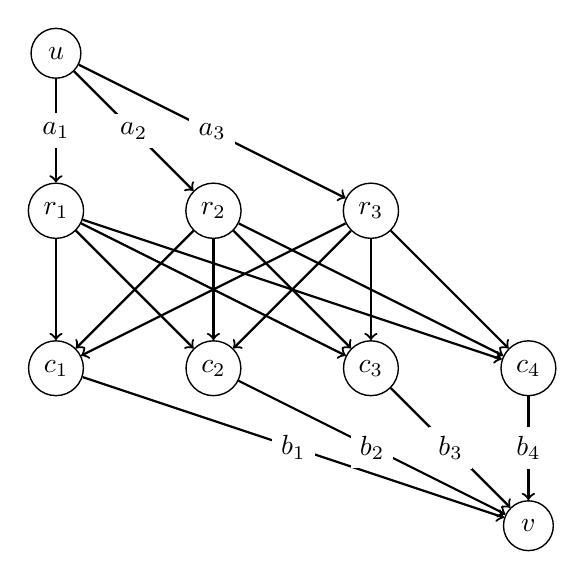
\begin{tikzpicture}[scale=2]
        \GraphInit[vstyle=Normal]
        \Vertex[x=0,y=0,L=$u$]{U}
        \Vertex[x=0,y=-1,L=$r_1$]{R1}
        \Vertex[x=1,y=-1,L=$r_2$]{R2}
        \Vertex[x=2,y=-1,L=$r_3$]{R3}
        \Vertex[x=0,y=-2,L=$c_1$]{C1}
        \Vertex[x=1,y=-2,L=$c_2$]{C2}
        \Vertex[x=2,y=-2,L=$c_3$]{C3}
        \Vertex[x=3,y=-2,L=$c_4$]{C4}
        \Vertex[x=3,y=-3,L=$v$]{V}
        \Edge[style={->},label=$a_1$](U)(R1)
        \Edge[style={->},label=$a_2$](U)(R2)
        \Edge[style={->},label=$a_3$](U)(R3)
        \Edge[style={->},label=$b_1$](C1)(V)
        \Edge[style={->},label=$b_2$](C2)(V)
        \Edge[style={->},label=$b_3$](C3)(V)
        \Edge[style={->},label=$b_4$](C4)(V)
        \Edge[style={->}](R1)(C1)
        \Edge[style={->}](R1)(C2)
        \Edge[style={->}](R1)(C3)
        \Edge[style={->}](R1)(C4)
        \Edge[style={->}](R2)(C1)
        \Edge[style={->}](R2)(C2)
        \Edge[style={->}](R2)(C3)
        \Edge[style={->}](R2)(C4)
        \Edge[style={->}](R3)(C1)
        \Edge[style={->}](R3)(C2)
        \Edge[style={->}](R3)(C3)
        \Edge[style={->}](R3)(C4)
      \end{tikzpicture}
    \end{center}
    \caption{A transportation network}
    \label{fig:transport}
  \end{figure}
\end{example}
\begin{definition}
  [Flow]
  A flow in a network $(N,A)$ with source $u$ and target $v$ is a function $f:A\to \RR_{\geq 0}$ whose value $f(x,y)$ at an arc $(x,y)\in A$ is known as the flow through the arc $(x,y)$.
  It is assumed to satisfy the condition that the flow through any vertex other than the source or sink of the network is $0$:
  \begin{equation}
    \label{eq:net-zero}
    \tag{*}
    \sum_{\{y\mid (x,y)\in A\}}f(x,y) - \sum_{\{y\mid (y,x)\in A\}} f(y,x) = 0 \text{ for all } x\in N-\{u,v\}.
  \end{equation}
  For subsets $M_1$ and $M_2$ of $N$ we use the shorthand:
  \begin{displaymath}
    f(M_1,M_2) = \sum_{\{(x,y)\in M_1\times M_2 \mid (x,y)\in A\}} f(x,y).
  \end{displaymath}
  If $M_1$ is the singleton set $\{x\}$ we write $f(x,M_2)$ for $f(M_1,M_2)$.
  Similarly if $M_2=\{y\}$ we write $f(M_1,y)$ for $f(M_1,M_2)$.
  Thus the equation \eqref{eq:net-zero} can be written as:
  \begin{displaymath}
    f(x,N)-f(N,x)=0 \text{ for every } x\in N.
  \end{displaymath}
  The \emph{value} of the flow is defined as the net flow out of the source $u$:
  \begin{displaymath}
    w_f = f(u,N) - f(N,u).
  \end{displaymath}
\end{definition}
\begin{exercise}
  Show that, for any flow $f$ on a network $(N,A)$ with source $u$ and sink $v$, the net flow out of the source $u$ equals the net net flow into the sink $v$:
  \begin{displaymath}
    w_f=f(u,N)-f(N,u)=f(N,v)-f(v,N).
  \end{displaymath}
\end{exercise}
\begin{definition}
  [Capacity function]
  A capacity function on a network $(N,A)$ is a function $c:A\to (0,\infty]$ (the value $\infty$ is permitted).
  Given a capacity function, a \emph{feasible} flow is a flow on $(N,A)$ such that $f(x,y)\leq c(x,y)$ for every $(x,y)\in A$.
\end{definition}
The capacity of arcs are represented by edge labels.
Labels for edges with infinite capacity are omitted.
In Example~\ref{example:transportation-network}, set $c(u,r_i)=a_i$ for $i=1,\dotsc,r$ and $c(s_j,v)=b_j$ for $j=1,\dotsc,s$, and all remaining arcs to have infinite capacity.
See Figure~\ref{fig:transport} for the visualization of this capacity function.

Given a network $(N,A)$ with a capacity function $c:A\to (0,\infty]$, the maximal flow problem is to maximize $v_f$ among all feasible flows on $(N,A)$ with capacity $c$.

Thus the max-flow problem has variables $f(x,y)$, for $(x,y)\in A$, and a variable $w$ (representing the value of the flow), and is given by:
\begin{equation}
  \label{eq:max-flow}
  \tag{F}
  \begin{array}{rll}
    f(x,N)-f(N,x)&=0 &\text{ for every $x\in N-\{u,v\}$},\\
    f(u,N)-f(N,u)-w&=0,&\\
    f(v,N)-f(N,v)+w&=0,&\\
    f(x,y)&\leq c(x,y)&\text{ for every $(x,y)\in A$}\\
    \hline
    \text{maximize } & f(u,N)-f(N,u). &
  \end{array}
\end{equation}

Let us consider the program dual to \eqref{eq:max-flow}.
It has a variable $\tau(x)\in \RR$ for $x\in N$, and a variable $\gamma(x,y)\geq 0$ for every $(x,y)\in A$.
For every $(x,y)$ in $A$ it has the constraint:
\begin{equation}
  \tag{DF}
  \label{eq:dual-flow}
  \begin{array}{rl}
    \tau(x)-\tau(y)+\gamma(x,y) & \geq 0 \\
    \tau(v)-\tau(u)& \geq 1.
  \end{array}
\end{equation}
and objective:
\begin{displaymath}
  \text{minimize } \sum_{(x,y)\in A} c(x,y)\gamma(x,y).
\end{displaymath}
\begin{definition}
  Let $(N,A)$ be a network, and $x,y\in N$.
  A \emph{path} from $x$ to $y$ is a sequence:
  \begin{displaymath}
    x=x_0,x_1,\dotsc,x_n=y \text{ such that } (x_{i-1},x_i)\in A \text{ for all }i=1,\dotsc,n.
  \end{displaymath}
\end{definition}
\begin{exercise}
  Use the duality theorem to show that if there is no path from $u$ to $v$ in $A$, then the maximum value of a feasible flow is is $0$.
\end{exercise}
\begin{definition}
  A \emph{cut} of the network $(N,A)$ is a partition $N=X\sqcup \bar X$ of its nodes such that $u\in X$ and $v\in \bar X$.
  The capacity $c(X,\bar X)$ of the cut is defined as:
  \begin{displaymath}
    c(X,\bar X) = \sum_{\{(x,y)\in A\mid x\in X,y\in \bar X\}} c(x,y).
  \end{displaymath}
\end{definition}
\begin{lemma}
  If $N=X\sqcup \bar X$ is a cut of $N$, then the value of any feasible flow is bounded above by $c(X,\bar X)$.
\end{lemma}
\begin{proof}
  Define
  \begin{displaymath}
    \gamma(x,y)=
    \begin{cases}
      1 & \text{if } x\in X,y\in \bar X,\\
      0 & \text{otherwise}.
    \end{cases}
  \end{displaymath}
  Define $\tau(x)=0$ for $x\in X$ and $\tau(x)=1$ for $x\in \bar X$.
  Then $\tau$ and $\gamma$ define a feasible solution for \eqref{eq:dual-flow}.
  The value of the objective is $c(X,\bar X)$, so this must be an upper bound for \eqref{eq:max-flow}.
\end{proof}
\begin{lemma}
  \label{lemma:augmentation}
  Let $f$ be a feasible flow.
  Define a new network $(N,A_f)$ by:
  \begin{displaymath}
    (x,y) \in A_f \text{ if }
    \begin{cases}
      (x,y)\in A \text{ and } f(x,y)<c(x,y), \text{ or}\\
      (y,x)\in A \text{ and } f(x,y)>0.
    \end{cases}
  \end{displaymath}
  If there is no path from $u$ to $v$ in $(N,A_f)$, then $f$ is a feasible flow of maximum value.
\end{lemma}
\begin{proof}
  Let $X$ denote the set of all nodes $x\in N$ such that $(N,A_f)$ admits a path from $u$ to $x$.
  The flow from $X$ into $\bar X$ is:
  \begin{displaymath}
    f(X,\bar X) = \sum_{\{(x,y)\in A\mid x\in X,y\in \bar X\}} f(x,y)-\sum_{\{(x,y)\in A\mid x\in \bar X,y\in X\}} f(x,y) = w_f.
  \end{displaymath}
  Since no point from $X$ has path to any point in $\bar X$ in the network $(N,A_f)$, we must have:
  \begin{gather*}
    f(x,y) = c(x,y) \text{ for all } (x,y)\in A, x\in X,y\in \bar X,\\
    f(x,y) = 0 \text{ for all } (x,y)\in A, x\in \bar X,\in X.
  \end{gather*}
  Therefore $f(X,\bar X)=c(X,\bar X)$ is a common value of the objective functions of \eqref{eq:max-flow} and its dual \eqref{eq:dual-flow}, hence optimal for both by the duality theorem (Theorem~\ref{theorem:duality} of Chapter~\ref{cha:intro-lp}).
\end{proof}
We are now close to prving the main theorem of this section:
\begin{theorem}
  [Max flow-min cut theorem]
  \label{theorem:max-flow-min-cut}
  The maximum value for feasible flows on a network $(N,A)$ with capacity $c$ is equal to the minimum capacity of its cuts.
\end{theorem}
\begin{proof}
  Let $f$ be a feasible flow.
  If it satisfies the hypothesis of Lemma~\ref{lemma:augmentation}, then it is optimal, and result follows.
  If not, let $P=(u=x_0,x_1,\dotsc,x_n=v)$ be a path in $(N,A_f)$ from $u$ to $v$.
  For each arc $(x,y)\in A_f$, define its \emph{spare capacity} as:
  \begin{displaymath}
    c'(x,y) =
    \begin{cases}
      c(x,y)-f(x,y) &\text{if } (x,y)\in A \text{ and } f(x,y)<c(x,y),\\
      f(y,x) &\text{if } (y,x)\in A \text{ and } f(y,x)>0.
    \end{cases}
  \end{displaymath}
  Let $m=\min\{c'(x_{i-1},x_i)\mid i=1,\dotsc,n\}$.
  By construction $m>0$.
  The \emph{augmentation of $f$ along $P$} is the flow $\tilde f$ for which
  \begin{align*}
    \tilde f(x_{i-1},x_i) & = f(x_{i-1},x_i) + m &\text{if $(x_{i-1},x_i)\in A$ and $f(x,y)<c(x,y)$},\\
    \tilde f(x_i,x_{i-1}) & = f(x_i,x_{i-1}) - m & \text{if $(x_i,x_{i-1})\in A$ and $f(x_i,x_{i-1})>0$},
  \end{align*}
  for each $i=1,\dotsc,n$, and all remaining values of $\tilde f$ are the same as those of $f$.
  Then $\tilde f$ is a feasible flow with value $w_f+m$, showing that $f$ was not optimal.
\end{proof}
The proof of the max flow-min cut theorem suggests an algorithm to find an optimal flow:
\begin{center}
  \textbf{Flow Augmentaiton Algorithm}
\end{center}
\begin{enumerate}
\item Begin with the zero flow $f\equiv 0$.
\item While the network $(N,A_f)$ admits a path $P$ from $u$ to $v$:
  \begin{itemize}
  \item   augment $f$ along $P$.
  \end{itemize}
\item Return $f$.
\end{enumerate}
\begin{theorem}
  Let $(N,A)$ be a networs with capacity funcion $c$ taking positive integer, or infinite values.
  If the set of values of feasible flows is bounded above, then the flow augmentation algorithm terminates in a finite number of steps and returns a flow with maximal value.
\end{theorem}
\begin{proof}
  The integrality of the capacities implies that the minimum spare capacity $m$ along a path of augmentation as in the proof of Theorem~\ref{theorem:max-flow-min-cut} is a positive integer.
  Therefore, during each run of the main loop of the algorithm the value of the resulting flow increases by $1$.
  Therefore, it the maximum possible value of all feasible flows is finite, it will be achieved in a finite number of steps.
\end{proof}
\begin{remark}
  The flow augmentation algorithm returns an integer-valued flow when the capacity function is integer-valued.
\end{remark}
Let $\Gamma$ be a bipartite graph with vertex set $N=U\coprod V$, and edge set contained in $U\times V$.
Suppose $\{(x_1,y_1),\dotsc,(x_k,y_k)\}$ is a matching in $\Gamma$, then any vertex cover of $\Gamma$ must contain at least one vertex from each of these edges.
Thus the minimum size of a vertex cover of $\Gamma$ must be at least as large as the maximum size of a matching.
The K\"onig-Egerv\'ary theorem states that these two quantities are equal:
\begin{theorem}
  For a biparite graph on vertex set $U\sqcup V$, the minimum size of a vertex cover equals the maximum number of edges in a matching in $\Gamma$.
\end{theorem}
\begin{proof}
  Let $N$ be the netowrk with nodes $U\sqcup V\sqcup \{u,v\}$, with arcs $(u,x)$ for all $x\in U$, $(x,v)$ for all $x\in V$, and $(x,y)$ for all $x\in U$ and $y\in V$ such that $\{x,y\}$ is an edge of $\Gamma$.
  Assign capacity $1$ to the arcs of the form $(u,x)$, $x\in V$ and $(x,v)$, $x\in U$.
  Allow the arcs joining $U$ to $V$ infinite capacity.

  A maximal value flow in $(N,A)$ corresponds to a maximal matching in $\Gamma$ (with flow of $1$ along the arcs corresponding to the edges in the matching).
  If $X\sqcup \bar X$ is a cut of finite capacity, it cannot contain any arc with infinite capacity.
  Therefore, there are no edges in $\Gamma$ between vertices from $X\cap U$ and $\bar X\cap V$, or in other words, every edge in $\Gamma$ corresponds to an arc with both end points in $X$ or both end points in $\bar X$.
  Thus $(\bar X\cap U)\cup (X\cap V)$ is a vertex cover.
  The capacity of this cut is $|\bar X\cap U|+|X\cap V|$.
  Thus the K\"onig Egerv\'ary theorem follows from the max flow-min cut theorem.
\end{proof}

\section{The supply-demand problem}
\label{sec:supply-demand-probl}

Consider a network $(N,A)$ with distinguished disjoint subsets $U$ and $V$ of nodes called supply nodes and demand nodes respectively.
Define functions $a:U\to [0,\infty)$ and $b:V\to [0,\infty)$ representing supply and demand values at these nodes.
Suppose also that a capacity function $c:A\to (0,\infty]$ is given.

The supply-demand problem is the following: determine if there exists a function $f:A\to [0,\infty)$ such that:
\begin{align}
  \tag{SD1}\label{eq:sd1}f(u,N)-f(N,u) & \leq a(u) \text{ for all }u\in U,\\
  \tag{SD2}\label{eq:sd2}f(v,N)-f(N,v) & \leq -b(v) \text{ for all }v\in V,\\
  \tag{SD3}\label{eq:sd3}f(x,N)-f(N,x) & = 0 \text{ for all }x\in N-(U\cup V),\\
  \tag{SD4}\label{eq:sd4}f(x,y) & \leq c(x,y) \text{ for all } (x,y)\in A.
\end{align}
This is a feasibilty problem, and so we take the objective function to be identically $0$.
The dual problem has variables $\tau(x)\in \RR$ for $x\in N$ and $\gamma(x,y)\geq 0$ for $(x,y)\in A$, satisfying:
\begin{displaymath}
  \tau(x)-\tau(y)+\gamma(x,y)\geq 0 \text{ for all } (x,y)\in A.
\end{displaymath}
The objective is:
\begin{displaymath}
  \text{minimize } \sum_{(x,y)\in A} c(x,y)\gamma(x,y)+\sum_{u\in U}a(u)\tau(u)-\sum_{v\in V}b(v)\tau(v).
\end{displaymath}
Suppose that $N=X\cup \bar X$ is any partition of $N$ into two parts.
As usual, let $\gamma(x,y)=1$ if $x\in X$ and $y\in \bar X$, and $0$ otherwise.
Let $\tau(x)=0$ for $x\in X$ and $\tau(x)=1$ for $x\in \bar X$.
These are feasible values for the dual program, and the value of the objective function is:
\begin{displaymath}
  a(\bar X\cap U) - b(\bar X\cap V) + c(X,\bar X). 
\end{displaymath}
If the primal program were feasible, then the maximum value of its objective function, namely $0$, would be a lower bound for the objective function of the dual.
Therefore, if the supply demand problem has a feasible solution then:
\begin{equation}
  \label{eq:aggregate-supply}
  b(\bar X\cap V) - a(\bar X\cap U) \leq c(X,\bar X) \text{ for every cut } N=X\cup \bar X.
\end{equation}
In other words, for every subset $\bar X$ of $N$, the shortfall in supply from nodes in $\bar X$ against demand from nodes in $\bar X$ cannot exceed the amount that can be supplied accross the cut $X\to \bar X$.
\begin{theorem}
  [Gale's supply-demand theorem]
  \label{theorem:supply-demand}
  The supply-demand problem has a feasible solution if and only if the condition \eqref{eq:aggregate-supply} is satisfied.
\end{theorem}
\begin{proof}
  Enlarge the network $(N,A)$ to $(N^*,A^*)$, where $N^*=N\cup\{u_0,v_0\}$, and $A^*=A\cup\{(u_0,u)\mid u\in U\}\cup \{(v,v_0)\mid v\in V\}$.
  For any cut $N^*=X^*\cup \bar X^*$, let $X=X^*\cap N$ and $\bar X = \bar X^*\cap N$.
  \begin{align*}
    c(X^*,\bar X^*) & = a(\bar X\cap U) + b(X\cap V) + c(X,\bar X)\\
                    & = a(\bar X\cap U) - b(\bar X\cap V) + c(X,\bar X) + b(V)\\
                    & \geq b(V)=c(\{u_0\}\cup N,\{v_0\}), 
  \end{align*}
  the last line being the capacity of the cut $(\{u_0\}\cup N,\{v_0\})$ separting $v_0$ from all the nodes in $N^*$.
  Therefore $(\{u_0\}\cup N,\{v_0\})$ is a cut in $(N^*,A^*)$ of minimum capacity $b(V)$.
  It follows that $(N^*,A^*)$ has a feasible flow with value $b(V)$.
  The restriction of this flow to $(N,A)$ is a feasible solution to the supply-demand problem.
\end{proof}
\begin{remark}
  If the functions $a$ and $b$ are integer-valued, then the supply-demand problem has an integer-valued feasible solution.
\end{remark}
\begin{corollary}
  Given vectors $\aa\in \RR^r$, $\bb\in \RR^s$ with positive coordinates having the same sum, let $\NN_{\aa\bb}$ denote the set of all $r\times s$ matrices $x_{ij}$ such that
  \begin{gather*}
    0\leq x_{ij}\leq 1 \text{ for all }1\leq i\leq r,1\leq j\leq s,\\
    \sum_{j=1}^s x_{ij} =  a_i \text{ for all } 1\leq i\leq r,\\
    \sum_{i=1}^r x_{ij} =  b_j \text{ for all } 1\leq j\leq s.
  \end{gather*}
  Then $\NN_{\aa\bb}$ is non-empty if and only if, for every subset $R\subset [r]$ and every subset $S\subset [s]$,
  \begin{displaymath}
    \sum_{j\in S} b_j - \sum_{i\in R} a_i \leq (r-|R|)|S|.
  \end{displaymath}
  Moreover, $\NN_{\aa\bb}$ is non-empty if and only if it has an integer point.
\end{corollary}
\begin{proof}
  Consider a network $(N,A)$ whose set $N$ of nodes is the disjoint union of $[r]$ and $[s]$.
  Let $U=[r]$ and $V=[s]$.
  Let $A=\{(i,j)\mid i\in [r],j\in [s]\}$.
  Define $c(i,j)=1$, $a(i)=a_i$, $b(j)=b_j$ for $i\in [r]$ and $j\in [s]$.
  Let $f$ be a feasible solution to this supply demand problem.
  Setting $x_{ij}=f(i,j)$ gives a point in $\NN_{\aa\bb}$.

  By Theorem~\ref{theorem:supply-demand}, this exists if and only if, for every subset $X\subset [r]\sqcup [s]$,
  \begin{displaymath}
    b(\bar X\cap [s]) - a(\bar X\cap [r]) \leq c(X,\bar X).
  \end{displaymath}
  setting $R=\bar X\cap [r]$ and $S=\bar X\cap [s]$ gives the condition in the theorem.
\end{proof}
\begin{corollary}
  \label{cor:aggregate-supply}
  There exists a function $f:A\to [0,\infty)$ satisfying \eqref{eq:sd1}--~\eqref{eq:sd4} if and only if, for every subset $V'\subset V$, there exists a function $f_{V'}:A\to [0,\infty)$ satisfying \eqref{eq:sd1}, \eqref{eq:sd3}, \eqref{eq:sd4} such that
  \begin{equation}
    \label{eq:V'}
    \tag{SD5}
    f_{V'}(N,V')-f_{V'}(V',N)\geq b(V').
  \end{equation}
\end{corollary}
\begin{remark}
  The inequality \eqref{eq:V'} says that, for every subset $V'$ of demand nodes, there exists a function satisfying the supply conditions, the capacity conditions, and the ``flow condition'' \eqref{eq:sd3} which meets the aggregate demand of $V'$ (but not necessarily the node-by-node demands).
\end{remark}
\begin{proof}
  If $f$ satisfies \eqref{eq:sd1}--~\eqref{eq:sd4}, then it obviously satisfies \eqref{eq:V'}.

  Conversely, suppose such an $f_{V'}$ exists for every $V'\subset V$.
  Let $N=X\cup \bar X$ be a partition.
  Take $V'=V\cap \bar X$, and let $N_0=N-(U\cup V)$.
  Then, using \eqref{eq:sd1}, \eqref{eq:sd3}, and \eqref{eq:V'} we have:
  \begin{align*}
    -a(U\cap\bar X)&\leq f_{V'}(N,U\cap \bar X)-f_{V'}(U\cap\bar X, N),\\
    0 & = f_{V'}(N,N_0\cap \bar X)-f_{V'}(N_0\cap\bar X, N),\\
    b(V\cap \bar X) & \leq f_{V'}(N,V\cap \bar X)-f_{V'}(V\cap\bar X,N).
  \end{align*}
  Adding up gives:
  \begin{displaymath}
    b(V\cap\bar X)-a(U\cap\bar X) \leq f_{V'}(N,\bar X) - f_{V'}(\bar X, N) = f_{V'}(X,\bar X)-f_{V'}(\bar X,X).
  \end{displaymath}
  Finally \eqref{eq:sd4} implies that $f_{V'}(X,\bar X)-f_{V'}(\bar X,X)\leq c(X,\bar X)$.
  Thus the the inequality \eqref{eq:aggregate-supply} is satisfied and the corollary follows from Theorem~\ref{theorem:supply-demand}.
\end{proof}
A dual version of Corollary~\ref{cor:aggregate-supply} is
\begin{corollary}
  \label{cor:aggregate-demand}
  There exists a function $f:A\to [0,\infty)$ satisfying \eqref{eq:sd1}--~\eqref{eq:sd4} if and only if, for every subset $U'\subset U$, there exists a function $f_{U'}:A\to [0,\infty)$ satisfying \eqref{eq:sd2}, \eqref{eq:sd3}, \eqref{eq:sd4} such that
  \begin{equation}
    \label{eq:U'}
    \tag{$\text{SD5}'$}
    f_{U'}(U',N)-f_{U'}(N,U')\leq a(U').
  \end{equation}
\end{corollary}
\begin{exercise}
  Prove Corollary~\ref{cor:aggregate-demand}.
\end{exercise}
\begin{example}
  [Hall's Marriage Theorem]
  Let $U=\{1,\dotsc,r\}$, $V=\{,1',\dotsc,r'\}$.
  Let $\Gamma$ be a bipartite graph with vertex set $U\sqcup V$,
  Hall's marriage theorem says that $\Gamma$ contains a perfect matching if and only if, for every $V'\subset V$, there exists $U'\subset U$ such that $|U'|=|V'|$ and every vertex in $V$ is connected to at least one vertex in $U'$.
  
  Hall's marriage theorem is a special case of Corollary~\ref{theorem:supply-demand}.
  To see this, let $N=U\sqcup V$, $A=\{(i,j)\mid \text{$i$ is connected to $j$ in $\Gamma$}\}$.
  Set the capacity of each arc to be $1$.
  Let $\aa=\bb=(1,\dotsc,1)$, the all-ones vector.
  Then an integer solution to the supply demand problem is a perfect matching.
  Suppose, for every subset $V'\subset V$, there exists $U'\subset U$ such that $|U'|= |V'|$ and for every $x\in U'$, there exists $y\in V'$ such that $(x,y)\in A$.
  Set $f_{V'}(x,y)=1$ for each such arc.
  Then $f_{V'}$ satisfies the conditions in Corollary~\ref{cor:aggregate-supply}, so that there exists a feasible solution to the supply demand problem.
\end{example}
Given a vector $\aa\in \RR^r$, let $\aa^\downarrow$ denote the vector obtained from $\aa$ by replacing its entries in weakly decreasing order.
Let $a^\downarrow_i$ denote the $i$th coordinate of $\aa^\downarrow$ (the $i$th \emph{order statistic} of $\aa$).
\begin{definition}
  \label{definition:majorization}
  Given two vectors $\aa\in \RR^r$ and $\bb\in \RR^s$, we say that $\aa$ \emph{majorizes} $\bb$ if, $\aa$ and $\bb$ have the same sum, and for every $1\leq k\leq r$,
  \begin{displaymath}
    \sum_{i=1}^k a^\downarrow_i \geq \sum_{i=1}^k b^\downarrow_i. 
  \end{displaymath}
  We write $\aa\rhd \bb$.
\end{definition}
A visual representation of a non-negative integer vector $\aa\in \RR^r$ is by its \emph{Young diagram}.
This is a configuration of $r$ left-justified rows of boxes, the $i$th row consisting of $a_i$ boxes.
For example, if $\aa=(3,1,2,2)$, then the Young diagram is:
\begin{displaymath}
  \ydiagram{3,1,2,2}
\end{displaymath}
\begin{definition}
  [Conjugate of an integer vector]
  Given $\aa\in \RR^r$, Define $\aa'=(a'_1,a'_2,\dotsc)$ by $a'_1+\dotsc + a'_k=\sum_{i=1}^r \min(a_i,k)$.
  Thus $a'_k$ is the number of boxes in the $k$th column of the Young diagram of $\aa$.
  Then $\aa'$ is an integer partition, known as the \emph{conjugate} of $\aa$.
\end{definition}
For example, the conjugate of $(3, 1, 2, 2)$ is $(4,3,1)$.
Note that rearranging the coordinates of $\aa$ does not change its conjugate.
This the conjugate of $(3,2,1,1)$ is also $(4,3,1)$.
\begin{exercise}
  If $\aa$ is an integer partition, then show that $(\aa')'=\aa$.
\end{exercise}
\begin{theorem}
  [Gale-Ryser]
  \label{theorem:gale-ryser}
  The polytope $N_{\aa\bb}$ is non-empty if and only if $\aa'\rhd \bb$.
\end{theorem}
Suppose $V'\subset V$.
A flow $f_{V'}$ which satisfies \eqref{eq:sd1}, \eqref{eq:sd3}, and \eqref{eq:sd4} of maximum value is obtained by simply supplying as much as possible from each $a_i$ to $V'$.
If $|V'|=k$, then $f_{V'}(u_i,V')=\min(a_i,k)$.
Summing over all $u\in U$ gives $f_{V'}(N,V')=f_{V'}(U,V')=\sum_{i=1}^r\min(a_i,k)$.
The condition \eqref{eq:V'} becomes:
\begin{equation}
  \label{eq:gr}
  \sum_{i=1}^k \min(a_i,k)\geq \sum_{j\in V'} b_j \text{ for every } V'\subset V \text{ with } |V'|=k.
\end{equation}
Then the left hand side of \eqref{eq:gr} is the number of boxes in the first $r$ columns of the Young diagram of $a$.
The condition \eqref{eq:gr} becomes:
\begin{displaymath}
  \sum_{i=1}^k a'_i \geq \sum_{j\in V'}b_j \text{ for every $V'\subset V$ with $|V'|=k$}.
\end{displaymath}
Then the above inequalities are equivalent to:
\begin{displaymath}
  \sum_{i=1}^k a'_i \geq \sum_{i=1}^k b^{\downarrow}_i.
\end{displaymath}
In other words, the partition $\aa'\rhd \bb$.
\begin{exercise}
  Let $\aa\in \RR^r$ and $\bb\in \RR^s$ be non-negative integer vectors with equal sum $d$.
  Reinterpret the Gale-Ryser theorem in the following forms:
  \begin{enumerate}
  \item There exist set partitions $[d]=R_1\sqcup \dotsb R_r=S_1\sqcup\dotsb\sqcup S_s$ such that $|R_i|=a_i$ for each $i$, and $|S_j|=b_j$ for each $j$, and $|A_i\cap B_j|\leq 1$ if and only if $\aa'\rhd \bb$.
  \item There exists a bipartite simple graph on vertex set $[r]\sqcup [s]$ such that the degree of each $i\in [r]$ is $a_i$ and the degree of $j\in [s]$ is $b)j$ if and only if $\aa'\rhd \bb$.
  \end{enumerate}
\end{exercise}

\section{The Hitchcock Problem}
\label{sec:hitchcock-problem}

Given vectors $\aa\in \ZZ_{\geq 0}^r$ and $\bb in \ZZ_{\geq 0}^s$ with the same sum, and a \emph{cost array} $(a_{ij})_{r\times s}$, the Hitchcock problem is the following linear program in variables $f_{ij}\geq 0$:
\begin{equation}
  \tag{H}
  \label{eq:hitchcock}
  \begin{array}{rcl}
    -\sum_{j=1}^s f_{ij} & \geq & - a_i \text{ for }i=1,\dotsc,r,\\
    \sum_{i=1}^r f_{ij} & \geq & b_j \text{ for }j=1,\dotsc,s,\\
    \hline
    \text{minimize} && \sum_{i=1}^r\sum_{j=1}^s a_{ij}f_{ij}.
  \end{array}
\end{equation}
The constraints are like in the supply demand problems in Section~\ref{sec:supply-demand-probl}, but now there is an ibjective function with positive coefficients.

The dual program has variables $\alpha_i>0$ for $i=1,\dotsc,r$ and $\beta_j\geq 0$ for $j=1,\dotsc,s$, and is given by:
\begin{equation}
  \tag{DH}
  \label{eq:dual-hitch}
  \begin{array}{rcl}
    -\alpha_i + \beta_j & \geq & a_{ij},\\
    \text{maximize} && -\sum_{i=1}^r a_i\alpha_i + \sum_{j=1}^s b_j\beta_j.
  \end{array}
\end{equation}

Suppose $(\alpha_1,\dotsc,\alpha_r,\beta_1,\dotsc,\beta_s)$ is a feasible solution for \eqref{eq:dual-hitch}, and $(f_{ij})$ is a feasible solution for \eqref{eq:hitchcock} such that:
\begin{equation}
  \label{eq:tight}
  -\alpha_i + \beta_j < a_{ij} \implies f_{ij}=0.
\end{equation}
Then,
\begin{align*}
  \sum_{i=1}^r \sum_{j=1}^s a_{ij}f_{ij} & = \sum_{-\alpha_i+\beta_j<a_{ij}} a_{ij}f_{ij} + \sum_{-\alpha_i+\beta_j=a_{ij}} a_{ij}f_{ij}\\
                                         & = 0 + \sum_{-\alpha+\beta_j=a_{ij}} (-\alpha_i+\beta_j)f_{ij}\\
  & = -\sum_{i=1}^r \alpha_i a_i + \sum_{j=1}^s \beta_jb_j.
\end{align*}
Thus we have feasible points for \eqref{eq:hitchcock} and \eqref{eq:dual-hitch} where where the objective functions coincide, hence are optimal.

A strategy to solve the Hithcock problem is to try and find such a pair of solutions.
Begin with an obvious feasible solution to \eqref{eq:dual-hitch}: Take $\alpha_i=0$ for all $i$, and $\beta_j = \min\{a_{ij}\mid i=1,\dotsc,r\}$ for $j=1,\dotsc,s$.
Now use the flow augmentaion algorithm on the network $N^*$  from the proof of Theorem~\ref{theorem:supply-demand} to try and find a feasible solution with $f_{ij}\geq 0$ to:
\begin{equation}
  \label{eq:2}
  \begin{array}{rcl}
    -\sum_{j=1}^s f_{ij} & \geq & - a_i \text{ for }i=1,\dotsc,r,\\
    \sum_{i=1}^r f_{ij} & \geq & b_j \text{ for }j=1,\dotsc,s,\\
    f_{ij} & = & 0 \text{ if } -\alpha_i+\beta_j = a_{ij}.
  \end{array}
\end{equation}
This is a supply demand problem in a modified transportation network (Example~\ref{example:transportation-network}) where some of the arcs $(i,j')$ are blocked.

If such a solution exists, then, as explained above, we have feasible solutions to \eqref{eq:hitchcock} and \eqref{eq:dual-hitch} with equal values of their objective functions, and we are done.

Otherwise, proceeding as in the proof of Lemma~\ref{lemma:augmentation}, Let $X\subset N^*$ denote the set of nodes reachable from $u_0$ in the modified transportaion network where arcs $(i,j')$ are blocked when $-\alpha_i+\beta_j<a_{ij}$.
Increase $\alpha_i$ and $\beta_j$ by $1$ for all the nodes in $\bar X$.
Since all the arcs between $X$ and $\bar X$ had slack ($-\alpha_i+\beta_j<a_{ij}$ when $i\in X$ and $j'\in \bar X$), the modified values of the dual variable are still feasible.

Now go back and to solving \eqref{eq:2} with the modified dual variables.
Continue this process unitl either an optimal common value for the objective functions of \eqref{eq:hitchcock} and \eqref{eq:dual-hitch} are found.
If this algorithm fails to produce a flow even when $-\alpha_i+\beta_j=a_{ij}$ for all $i,j$, then the transportation problem itself is infeasible. 
\section{The cost minimization problem}
\label{sec:cost-minim-probl}
The Hitchcock problem is a special case of a more general minimal cost supply-demand problem, where the constraints \eqref{eq:sd1}--~\eqref{eq:sd4} of Section~\ref{sec:supply-demand-probl} on variables $f(x,y)\geq 0$ are paired with the objective:
\begin{displaymath}
  \text{maximize } \sum_{(x,y)\in A} a(x,y) f(x,y).
\end{displaymath}
Assume that the cost function $a:A\to [0,\infty)$ and the capacity function $c:A\to (0,\infty]$ are integer valued (but $c$ is allowed infinite values).
Also the supply and demand constrains $a$ and $b$ are integer-valued.

We modify the problem a little bit for convenience.
Add nodes $u_0$ and $v_0$ to the network, and connect $u_0$ to each node $u\in U$ by an arc of capacity $a(u)$ and cost $0$.
Connect $v_0$ to each node $v\in V$ with an arc of capacity $b(v)$ and cost $0$.
Denote the resulting network by $(N^*,A^*)$.
We introduce an unrestricted variable $w$ for the value of the flow.
The modified program has variables $f(x,y)\geq 0$ for each $(x,y)\in A^*$, and a variable $w\in \RR$, and is given by:
\begin{equation}
  \tag{C}
  \label{eq:min-cost}
  \begin{array}{rcl}
    f(u,N)-w&=&0,\\
    f(x,N)-f(N,x)&=&0 \text{ for }x\in N^*-\{u,v\},\\
    f(v,N)+w&=&0,\\
    f(x,y)&\leq&c(x,y) \text{ for }(x,y)\in A^*.\\
    \hline
    \text{minimize}&&pw-\sum_{(x,y)\in A} a(x,y)f(x,y).
  \end{array}
\end{equation}
The quantity $p$ is a parameter, set to take values $0,1,2,\dotsc$ sequentially.
As $p$ increases, minimal cost flows of successively higher values are obtained, and for $p$ sufficiently large, flows of maximal value are obtained (without reference to the cost function).
The dual has variables $\tau(x)\in \RR$ for $x\in N^*$, and $\gamma(x,y)\geq 0$ for $(x,y)\in A^*$ and is given by:
\begin{equation}
  \label{eq:DC}
  \tag{DC}
  \begin{array}{rcl}
    -\tau(u)+\tau(v) & = & p,\\
    \tau(x)-\tau(y)+\gamma(x,y)&\geq& -a(x,y) \text{ for }(x,y)\in A^*,\\
    \hline
    \text{maximize}&&-\sum_{(x,y)\in A^*} c(x,y)\gamma(x,y).
  \end{array}
\end{equation}
\begin{lemma}
  \label{lemma:cost-optimality}
  If $f$, $\tau$ and $\gamma$ are feasible solutions to \eqref{eq:min-cost} and \eqref{eq:DC} which satisfy:
  \begin{align*}
    \tau(u)=0, \tau(v)=p,&\\
    \tau(x)-\tau(y)+\gamma(x,y)>-a(x,y) & \implies f(x,y)=0,\\
    \gamma(x,y)>0 & \implies f(x,y)=c(x,y),
  \end{align*}
  Then they have the same value of the the objective function, hence are optimal.
\end{lemma}
\begin{proof}
  We have:
  \begin{align*}
    pw-\sum_{(x,y)\in A^*} a(x,y)f(x,y) & = pw-\sum_{(x,y)\in A^*} (\tau(x)-\tau(y)+\gamma(x,y))f(x,y)\\
                                        & = pw - \sum_{(x,y)\in A^*} (\tau(x)-\tau(y))f(x,y)\\&\phantom{=} - \sum_{(x,y)\in A^*} \gamma(x,y)c(x,y)\\
                                        & = pw - \tau(x)(f(x,N) - f(N,x)) - \sum_{(x,y)\in A^*}\gamma(x,y)c(x,y)\\
    & = -\sum_{(x,y)\in A^*}\gamma(x,y)c(x,y),
  \end{align*}
  whence the objectives of \eqref{eq:min-cost} and \eqref{eq:DC} are equal.
\end{proof}
It is now more or less clear how to solve the cost minimization algorithms:

Begin with $\tau\equiv 0$, $\gamma\equiv 0$, $f\equiv 0$.
The conditions of Lemma~\ref{lemma:cost-optimality} are satisfied.

Suppose, at a given stage of the algorithm we have $\tau$, $\gamma$, and $f$ satisfying the conditions of Lemma~\ref{lemma:cost-optimality}, with $p=\tau(v)$.
Construct an auxilliary network $(N^*,A^\dagger)$ with capacity $c^\dagger$ as follows:
For $x,y\in N^*$, $(x,y)$ is an arc of $A^\dagger$ if either:
\begin{itemize}
\item $(x,y)\in A$, $\tau(x)-\tau(y)+\gamma(x,y)=-a(x,y)$ and $f(x,y)<c(x,y)$.
  Set $c^\dagger(x,y)=c(x,y)-f(x,y)$.
\item $(y,x)\in A$, $f(y,x)>0$, $\gamma(x,y)=0$.
  Set $c^\dagger(x,y)=f(y,x)$.
\end{itemize}
If there exists a path from $u$ to $v$ in $(N^*,A^\dagger)$, augment $f$ along this path.
Because of the way in which we have chosen the nodes of the auxilliary network, the augemented flow still satisfies the conditions ot Lemma~\ref{lemma:cost-optimality}.
If there is no path from $u$ to $v$ in $(N^*,A^\dagger)$, then set $\tau'(x)=\tau(x)+1$ for every node $x\in N^*$ that is not reachable from $u$, and $\tau'(x) = \tau(x)$ for every node reachable from $u$.
We claim that:
\begin{displaymath}
  \tau'(y)-\tau'(x)<a(x,y)\implies f(x,y)=0.
\end{displaymath}
This can happen in two ways.
Either $\tau(y)-\tau(x)=\tau'(y)-\tau'(x)$, so $f(x,y)=0$.
Otherwise, $\tau'(y)=\tau(y)$ but $\tau'(x)=\tau(x)+1$.
So $x$ was not reachable from $u$ in $(N^*,A^\dagger)$, while $y$ was.
Then $f(x,y)$ must be $0$, since otherwise, $x$ would be reachable through $y$ since $(y,x)\in A^\dagger$.
We also claim that:
\begin{displaymath}
  \tau'(y)-\tau'(x)>a(x,y) \implies f(x,y)=c(x,y).
\end{displaymath}
The proof is a similar consideration of cases.

Thus, at each stage of the algorithm, either $p$ is incremented by $1$, or $w$ is incremented by a positive integer.
At each stage the flow $f_p$ maximizes the objective function of \eqref{eq:min-cost} for the current value of $p$.

Given a path $u=x_0,x_1,\dotsc,x_n=v$ such that either $(x_{i-1},x_i)\in A^*$ (forward arcs) or $(x_i,x_{i-1})\in A^*$ (reverse arcs), define the path cost to be the sum of the costs of the forward arcs minus the sum of the costs of the reverse arcs.
\begin{theorem}
  Once $p$ exceeds the maximum path cost of all paths from $u$ to $v$, then $f_p$ is a flow of minimum cost among all maximum value flows.
\end{theorem}
\begin{proof}
  If not, then $f_p$ is not a maximum value flow.
  An augmenting path in the auxilliary netowrk will have at least one forward arc $(x,y)$ such that $\tau(y)-\tau(x)<a(x,y)$ or at least one reverse arc $(y,x)$ such that $tau(y)-\tau(x)>a(x,y)$.
  Therefore $p=\tau(v)-\tau(u)$ will be strictly less than the path cost of this path, a contradiction.
\end{proof}

\bibliographystyle{abbrv}
\bibliography{refs}
\end{document}
